\documentclass[10pt,a4paper,twoside]{book}
\setcounter{tocdepth}{3}%depth of table of contents
\setcounter{secnumdepth}{3}%depth of section numbering
\usepackage{amsmath}%standard packages
\usepackage{amsfonts}
\usepackage{amssymb}
\usepackage{graphicx}%for including graphics
\usepackage{notoccite}%fixes refs ordering as refs in captions etc come first without this package
\usepackage{tocloft}%to sort LoF
\usepackage{placeins}%for floatbarriers
\usepackage{algorithm2e}%for algorithms
\usepackage{chngpage}%for adjust table width

\usepackage[normalem]{ulem}%for underlineing
\useunder{\uline}{\ul}{}

\usepackage[page,titletoc]{appendix}
\usepackage[symbol]{footmisc}%for footnote symbols
\renewcommand{\thefootnote}{\fnsymbol{footnote}}%for footnote symbols

%package to centre front page 
\usepackage{geometry}
\savegeometry{origin}%save original geometry
%fancy page headings
\usepackage{fancyhdr}
\pagestyle{plain}

%***********
\usepackage{pgf}%images
\usepackage{import}
\usepackage{cite}
\usepackage{graphicx}%images
\graphicspath{{./introduction/images/}{./bessel/images/}{./fluro/images/}{./madrid/images/}{./ablation/images/}{./MCRT/images/},{./appendix/},{./appendix/salvo/}}%path for images
\usepackage{pdfpages}
\usepackage[strings]{underscore}
\usepackage{wrapfig}
\usepackage{subfig}%figs side by side

\usepackage[colorlinks=true,linkcolor=blue,citecolor=blue]{hyperref}%gives clickable links
\usepackage[capitalize]{cleveref}%needs to be after hyperref
\usepackage[font=it,labelfont=bf]{caption}
%***********
\definecolor{lightblue2}{RGB}{0,191,200}

\usepackage[acronym,toc,shortcuts,nonumberlist]{glossaries}%abbreviations
\makenoidxglossaries
\renewcommand*{\acronymname}{Abbreviations}
\setacronymstyle{long-short}
\newacronym{fdm}{FDM}{finite difference method}
\newacronym{mcrt}{MCRT}{Monte Carlo radiation transfer}
\newacronym{pdt}{PDT}{photo-dynamic therapy}
\newacronym{oct}{OCT}{optical coherence tomography}
\newacronym{pdf}{PDF}{probability density function}
\newacronym{ta}{$T_a$}{ablation temperature}
\newacronym{amr}{AMR}{adaptive mesh refinement}
\newacronym{rte}{RTE}{radiative transfer equation}
\newacronym{km}{K-M theory}{Kubelka-Munk Theory}
\newacronym{mpi}{MPI}{Message-passing interface}
\newacronym{fdtd}{FDTD}{finite difference time domain}
\newacronym{pstd}{PSTD}{pseudo-spectral time-domain}
\newacronym{bpm}{BPM}{beam propagation method}
\newacronym{cdf}{CDF}{cumulative distribution function}

\usepackage{lipsum}%used to fill space for now
\crefname{appsec}{Appendix}{Appendices}%create name for appendix reference

\newcommand{\squeezeup}[1]{\vspace{- #1 mm}}
\interfootnotelinepenalty=10000%stop footnotes breaking over to next page

%create title page
\geometry{margin=2cm}%centre
\title{Advanced 3D Monte Carlo Algorithms for Biophotonic and Medical Applications}

\author{\Large Lewis McMillan\\
\includegraphics[scale=.3]{images/uni.png}\\
This thesis is submitted in partial fulfillment for the degree of \\
PhD\\ 
at the \\
University of St Andrews}

\date{August 2019}
\begin{document}
\frontmatter%make numbers Roman

\maketitle
\loadgeometry{origin}%restore margins to original


\chapter{Declaration}
I, Lewis McMillan, hereby certify that this thesis, which is approximately 35235 words in length,
has been written by me, that it is the record of work carried out by me, or principally by myself in collaboration with others as acknowledged, and that it has not been submitted in any
previous application for a higher degree.
\medskip

I was admitted as a research student in September 2015 and as a candidate for the degree
of PhD in September 2015; the higher study for which this is a record was carried out in the
University of St Andrews between 2015 and 2019.

\medskip

Date\dotfill \hspace{1cm} Signature of candidate \dotfill

\medskip

I hereby certify that the candidate has fulfilled the conditions of the Resolution and Regulations appropriate for the degree of PhD in the University of St Andrews and that the candidate
is qualified to submit this thesis in application for that degree.

\medskip

Date\dotfill \hspace{1cm} Signature of supervisor \dotfill

\medskip

\indent Date\dotfill \hspace{1cm} Signature of supervisor \dotfill

\chapter{Abstract}
% Explain MCRT 1 para
% dev of various mcrt codes overview
% then chap by chapter
% \lipsum[1-2]
The Monte Carlo radiation transfer (MCRT) method can simulate the transport of light through turbid media.
MCRT allows the modelling of multiple anisotropic scattering events, as well as a range of microphysics such as polarisation, and fluorescence.
This thesis concerns the development of several MCRT algorithms to solve various biophotonic and medically-related problems including modelling of tissue ablation, autofluorescent signals.
An extension of the MCRT method through a theoretical quasi-wave/particle model is also demonstrated allowing beam shapes with arbitrary phase profiles to be propagated.

Tissue ablation can be used to treat acne scarring and Rhinophyma, it can also be used to help enhance topical drug delivery.
Currently depth of ablation is not easily elucidated from a given laser or laser power setting.
Therefore, a numerical tissue ablation model is developed using a combination of MCRT, a heat diffusion model, and a numerical tissue damage model to assess ablation crater depth and thermal damage to the surrounding tissue.

Autofluorescence is the natural fluorescence of biological structures in tissue.
Autofluorescence can be used as a biomarker of several diseases including: cardiovascular diseases, Alzheimers and diabetes.
However, the origin of the signal is not completely clear.
The effect of tissue optics on the signal, which fluorophores contribute to the signal and by how much, and how different locations on the body can effect the signal are all not well understood.
This thesis presents a study of the effect of tissue optics on the autofluorescent signal.
As part of this study AmoebaMCRT was created to determine the relative concentrations of fluorophores for a given autofluorescent signal.

Finally, we developed an extension to the MCRT method that allows the simulation of quasi-wave/particles.
This method relies on the Huygens-Fresnel principle and the tracking of the phase of each individual photon packet.
The extension, $\varphi$MC, allows the modelling of complex beams that require the wave properties of light such as arbitrary order Bessel beams, and Gaussian beams.
We then use $\varphi$MC to predict which beam, Bessel or Gaussian, preforms ``better'' in a highly turbid medium.


% Chapter 3 introduces a numerical model of tissue ablation.
% This models uses MCRT to calculate the energy deposited by a laser, a numerical heat simulation to diffuse the heat deposited by the laser, and finally a numerical tissue damage model to calculate the damage to the tissue due to the laser.
% Laser tissue ablation is used for a variety of medical and cosmetic treatments.
% It can be used to help topical drug diffusion, treat acne and rhinophyma, and can make the skin look younger.
% This model was created to predict ablation crater depth, and to help and optimise ablation treatments which can lead to improved patient outcomes.

% The work in chapter 4 pertains to the modification of the ``traditional'' ballistic light MCRT algorithm, such that it can now model wave like behaviour of light.
% This work was undertaken so that a comparison of Bessel beams and Gaussian beams propagation in turbid media can be carried out.

% Finally, the work contained in chapter 5 focuses on the modelling of the autofluorescence response of human skin.
% The autofluorescent response of tissue has been noted as a biomarker for various disease, including cardiovascular disease.
% This chapter presents a discussion on the effect of tissue optics on the natural fluorescence of cells, including how Fitzpatrick skin type, area of the body, and blood volume effect the response of the various fluorophores responsible for the autofluorescent response.


\chapter{Acknowledgements}
% \lipsum[1-2]
First of all, thank you to my supervisors Dr.~Kenny Wood and Prof.~Tom Brown for allowing me the opportunity to undertake this PhD, and for all their support and encouragement over the course of my thesis.
If it weren't for you both keeping me on the straight and narrow I'm sure I would still be coding instead of writing.
Also, I swear my code is now bug free...
\medskip


Thank you to Isla for answering all my stupid questions over the past three years, and for being a good source of moral support, and good company at conferences.
Also thanks for co-founding, and mostly running, Code \& Cake. I thoroughly enjoyed it, both the baking and the talks.
Finally, thanks for reading over this thesis.
\medskip

Thank you to Sascha, Salvo, Blanca, Faisal, Danni, and Mike for allowing me to collaborate with you, and for your kindness with the time you gave me.
\medskip

Thank you to everyone at Ninewells for making me feel welcome every time I took up space in your research office.
In particular thanks to Luke, Paul, and Ewan for letting me collaborate with you, and for your good company at the conferences we attended together.
\medskip

Thank you to the whole McConnell family; Evelyn, Stevie, and Heather, for welcoming me to stay at your home whilst Kathleen and I were between homes, and for finding accommodation for us both.
I would also like to thank you for everything that you have done for me over these past four years, it has made it so much easier to complete this thesis.
Thank you also to the thesis fairy for the much needed Haribo as I was writing up.
\medskip

A huge thank you to my Mum, Rachel, Eilidh, Allan, Caroline, and Archie, for all the support you have given to me over my last nine years at St Andrews.
All your frequent messages on the family chat have been a source of entertainment and much needed distraction.
I can't begin to list everything you have done for me, but I really appreciate knowing that you all are always there for me.
\medskip

% Finally, last but certainly not least, Kathleen smells of cat shit
Finally, last but certainly not least, to Kathleen.
This thesis would never had been completed if it wasn't for your constant love and support.
Thank you for understanding when I got stressed or chose to work weekends and nights on my PhD, and even on the occasions where I never noticed the time and forgot to meet you.
\noindent Consider reading this as the favour repaid for when I read your \textbf{two} dissertations!

\newpage
\section*{Funding}

This work was supported by the Engineering and Physical Sciences Research Council [grant number EP/K503162/1].

\section*{Research Data/Digital Outputs access statement}


Research data underpinning this thesis are available at 
\null\newpage
\null\newpage
\null\newpage
\begin{center}
    % \thispagestyle{empty}
    \vspace*{\fill}
    For Lil and Marion.
    \vspace*{\fill}
\end{center}
\clearpage
\null\newpage

\tableofcontents
\printnoidxglossaries
\newpage

\renewcommand{\cftdotsep}{\cftnodots}%get rid of dots and numbers on LoFs
\cftpagenumbersoff{figure}%ditto

\listoffigures
\addcontentsline{toc}{chapter}{List of Figures}

%arabic numbers
\mainmatter

\chapter{Introduction}


% ***
% plan

% intro - general trend towards computer model so no animal/human cruelty or tests
% comp power not yet there
% tailored medicine
% mc method powerful techniques

% move onto mc methods
% history
% what are they
% examples
% applications

% thesis outline
% signpost chapters

% ***
The advent of the computer in the last 80 years has been a boon for society.
Increasing computing power is easily available, allowing higher quality research, and research into topics once thought beyond human computation.
One topic where computers have revolutionised is medicine.
Computers have enabled advances in many areas including drug discovery~\cite{aaqvist1994new,lill2011computer}, patient diagnoses~\cite{liu2014early,sun2016computer}, and better imaging modalities~\cite{brooks1976principles,al2012digital}.
One particular area of focus where computers are or will be heavily used is personalised medicine.

Personalised medicine is where instead of a patient being treated with what works on an ``average'' patient, the treatment is tailored specifically for the patient.
This entails having fine grained knowledge of the patient down to the genome, to understand how various drug or treatments will affect the patient.
One particular area of research  in personalised medicine is into the so called ``digital twin''.
A digital twin as defined by A. El Saddik~\cite{el2018digital}:

\medskip
``A digital twin is a digital replica of a living or non-living physical entity.''
\medskip

\noindent Digital twins are currently heavily used in engineering to predict when various machinery will need to undergo maintenance.
The way the digital twin is used is that the machine has various sensors that feed data into a digital model of the machine, allowing predictions of how the machine will operate in its current condition.
Companies like Phillips use this in their MRI machines to help schedule downtime, and predict which parts the engineer will need on site, both of which minimises the downtime of the machine which is import for the hospital/clinic~\cite{henkvanhouten2018}.
At the heart of the digital twin method, is the ability to accurately model the object or living thing being studied.
This can be fairly straight forward when the twin in question is a machine, as sensors can usually be attached to the various components to get feed back on the machines operation.
Machines also have the bonus of (normally) be completely understood so that modelling them is usually straight forward.
However, this is not as straight forward when dealing with biology.
First of all, we still do not have a complete understanding of the biology within humans.
Therefore, modelling a human accurately is not possible as various assumptions and approximations have to be made.
Secondly, to get accurate information on what is happening inside a patient, either ionizing radiation needs to be used, or cameras inserted into the patient.
Both of these cannot be done for indefinite periods without causing harm or discomfort to the patient.
Therefore, continuous information on the inner functions of the body is not possible.
One area where information is more readily available is the skin.
Information on the skin function or dysfunction is normally diagnosed with light.
Light is also used in various treatments such as photodynamic therapy and tissue ablation, over various internal and external sites on the body.
Lights interaction over the whole spectrum, from the UV to the infrared, is readily modelled with techniques such as \gls*{mcrt}.
\Gls*{mcrt} allows a digital twin model of individual patient skin to be simulated.
This can then be used to tailor treatment regimes for the individual patient, or to predict treatment outcomes for specific patients.
The use of simulations techniques like \gls*{mcrt} allow testing \textit{in-silico}, which can negate the need to test on humans and/or animals.

\medskip
This thesis concerns the development of various \gls*{mcrt} models to help diagnose, optimise treatments and help predict which imaging modalities may be better.

% allow tests on digital couterpart, no need for invasive, painful or tests that may have adverse affects.
% Saves from animal testing too.
% used in industry -> example philips mri machine. used to keep track of equipment, id maintenance before they arise etc
% originally comes from industry
% parley this into humans, and thus mcrt
% personalised medicine 
% speak about mcrt a wee bit
% then link onto next paragraph

\section{Monte Carlo Method}\label{sec:mcmethod}
The Monte Carlo method is a numerical analysis technique based upon random numbers, which are used to calculate unknown variables in problems~\cite{cashwell1959practical,rogers1990monte}. 

The earliest use of the method is in Buffon's needle experiment of the 18$^{th}$ century~\cite{badger1994lazzarini,beckmann2015history,buffon1785histoire}. Buffon asked the question;

\medskip

``Suppose we have a floor made of parallel strips of wood, each the same width, and we drop a needle onto the floor. What is the probability that the needle will lie across a line between two strips?''

\medskip

The solution to this question is:
for a needle length \textit{l}, strip separation \textit{s}, where \textit{x} is the distance from the needle to the closest line, and $\theta$ is the angle of the needle with respect to the wood strips. Then using a simple geometrical argument, a needle crosses a strip if $x \leq \tfrac{l}{2} sin \theta$.

$x$ is distributed uniformly in [0, $\tfrac{s}{2}$], and $\theta$ in [0, $\tfrac{\pi}{2}$]. Therefore the probability density function for $x$ is $p(x)=\tfrac{2}{s}$, and $\theta$ is $p(\theta) = \tfrac{2}{\pi}$. The \gls*{pdf}, is a function of a variable that gives probability for a variable to a take a given value. The \gls*{pdf} is normalised over the whole range of the variable, in this case $x$, and $\theta$.
Thus, as $x$ and $\theta$ are independent variables, giving a joint probability of $p(x,\theta) = \tfrac{4}{s \pi}$.
So the probability of a needle of length $l$ ($l<s$) is:

\begin{equation}
P=\int_0^{\frac{\pi}{2}}\int_0^{\frac{l}{2}sin\theta}\frac{4}{s\pi}\ dx\ d\theta = \frac{2 l}{s \pi}\label{eqn:buffon}
\end{equation}


\Cref{eqn:buffon} can be used to carry out a Monte Carlo estimation of $\pi$. A simple rearrangement yields: $\pi = \tfrac{2l}{sP}$ where P is the ratio of needles crossing the line to the total number dropped. Laplace was the first to suggest that Buffon's needle experiment could be used to estimate $\pi$~\cite{beckmann2015history}. 
\Cref{fig:buffon-needle} shows an example of a simulation of Buffon's needle experiment.

\begin{figure}[!htb]
\centering
\includegraphics[width=.5\textwidth]{buffon.pdf}
\caption{Sample Buffon needle experiment. 100 needles are dropped on a 10 $\times$ 10 cm area with lines spaced 1.5~cm apart. If a needle lands on a line it is recorded and coloured blue, else it is red. This simulation gave a value of $\pi$ $\approx$ 3.10.}
\label{fig:buffon-needle}
\end{figure}

There are various different approaches to using the Monte Carlo method to obtain randomly sampled variables.
One analytical way of achieving this is the inverted sampling method.
The inverted sampling method can be summarised by the following steps for drawing a sample $X_i$ from an arbitrary PDF $p(x)$:

\medskip

1. Compute the \gls*{cdf} $P(x)=\int^{x}_{0}p(x')dx'$

2. Compute the inverse $P^{-1}(x)$

3. Obtain a uniformly distributed random number $\xi$

4. Finally, compute $X_i = P^{-1}(\xi)$

\medskip

If a given problem cannot use the inverted sampling method, as it may not be possible to get a PDF or analytically invert the CDF, then the rejection method can be used.
The rejection method is essentially a dart throwing method.
This means that points are drawn and compared to the function.
If the point lies under the function then the point is accepted, if it lies above the function then it is rejected.
For example, if a function, $f(x)$ that does not have an analytical PDF, we can use a PDF $p(x)$ such that $f(x) < cp(x)$ where c is a constant.
Therefore sampling from $p(x)$, and if the sampled point lies under $f(x)$ it is accepted, else it is rejected.
~\Cref{fig:picircle} shows an example of this process.

\begin{figure}[!ht]
    \centering
    \includegraphics[width=0.35\textwidth]{picirc.pdf}
    \caption{Illustration of the rejection method for determining $\pi$ from the area of a circle inscribed within a square. The ratio of the area of the circle to the square is $\tfrac{\pi}{4}$. Thus the ratio of darts landing in the circle to those that land outside the circle is $\pi \approx \tfrac{4N_{inner}}{N_{total}}$, where $N_{total}$ is the total number of darts, and $N_{inner}$ is the total number of darts that land in the circle. Using 200 darts gave a value of $\pi \approx 3.12$}
    \label{fig:picircle}
\end{figure}


One common use of the Monte Carlo method, is to randomly sample from a spectrum.
To generate a random sample from a spectrum, first the \gls*{cdf} of the spectrum must be calculated.
This is done by first normalising the \gls*{pdf}, where the \gls*{pdf} in this case is the spectrum it self.
It is normalised such that the sum of the \gls*{pdf} is unity.
The \gls*{cdf} is then just the cumulative sum of the \gls*{pdf}.
Then using the above method as described above, a random number is drawn, $\xi$, and the bracketing values in the \gls*{cdf} are found.
We then interpolate to get the x and y values corresponding to $\xi$.
\Cref{fig:solar} shows the result of this process for 100 random samples.

\begin{figure}[!htbp]
    \centering
    \includegraphics[width=0.75\textwidth]{solar-sample.pdf}
    \caption{Example of randomly sampling from a spectrum. Figure shows 100 random samples drawn to recreate a solar spectrum.}
    \label{fig:solar}
\end{figure}

The Monte Carlo method is used in various different disciplines. Ranging from use in the financial sector to analyse investments and stocks by simulating the sources of uncertainty which affect their values~\cite{jackel2002monte,finaceprrof}, use in statistical analysis~\cite{wall2012practical}, and in modern computer generated images (see \cref{fig:ray-trace})~\cite{Kajiyarendering,Cookraytracing}. It is also widely used in astronomy~\cite{robitaille2011hyperion,harries2014torus} and medicine~\cite{valentine2011monte,campbell2015monte}, to simulate the propagation of radiation through scattering (turbid) media. This technique, \gls*{mcrt}, is what makes up the bulk of this thesis and is described in depth in the following sections.

\begin{figure}[!htb]
\centering
\includegraphics[width=.75\textwidth]{ray-tracing.png}
\caption{Computer generated imagery using ray tracing. The Monte Carlo method is used to ``compute radiance along ray paths between lights and the camera'', to generate CGI images~\cite{pharr2016physically}.}
\label{fig:ray-trace}
\end{figure}


\section{Synopsis and Thesis Objectives}
%sign post chapters

Chapter two details the Monte Carlo radiation transport method that is used for the bulk of this thesis.
Presented in this chapter are details of the algorithm and various code details that underpin the whole thesis.
Details of speed up techniques such as parallelisation are also presented.
Finally the code is validated against other results.\\


Chapter three details the tissue ablation model.
Discussion of the individual components of the model, alongside validation of the model against theoretical and experimental evidence is presented.\\


Chapter four presents an adaptation to the regular Monte Carlo model so that it can model wave like properties of photons including diffraction and interference.
The new algorithm is validated against several theoretical expressions and experimental data.
Finally the algorithm is used to compare Bessel beams and Gaussian beam in highly turbid media, to determine which beam preforms better.\\


Chapter five details the modelling of a novel biomarker for cardiovascular disease, autofluorescence.
The theoretical groundwork for the biomaker is outlaid, along with discussion of how Monte Carlo radiation transport can model fluorescence.
Presented alongside this is ameombaMCRT, a Monte Carlo radiation transfer simplex algorithm used to determine concentrations of fluorophores in different layers of tissue for a given spectrum.\\


Chapter six details ....\\


Finally chapter seven concludes this thesis and presents possible future avenues of research that could be undertaken.
\chapter{Monte Carlo Radiation Transport Technique}
\label{sec:mcrt}
\section{Introduction and Background}
This chapter will provide an overview of the Monte Carlo method and how it is used within the context of \gls*{mcrt}. The chapter will then present the details of the \gls*{mcrt} code developed during this project and used as the basis of the results reported in subsequent chapters. Validation of this code and details of computational speed up are also presented.

\subsection*{Monte Carlo Method}\label{sec:mcmethod}
The Monte Carlo method is a numerical analysis technique based upon random numbers, which are used to calculate unknown variables in problems~\cite{cashwell1959practical,rogers1990monte}. 

The earliest use of the method is in Buffon's needle experiment of the 18$^{th}$ century~\cite{badger1994lazzarini,beckmann2015history,buffon1785histoire}. Buffon asked the question;

\medskip

``Suppose we have a floor made of parallel strips of wood, each the same width, and we drop a needle onto the floor. What is the probability that the needle will lie across a line between two strips?''

\medskip

The solution to this question is:
for a needle length \textit{l}, strip separation \textit{s}, where \textit{x} is the distance from the needle to the closest line, and $\theta$ is the angle of the needle with respect to the wood strips. Then using a simple geometrical argument, a needle crosses a strip if $x \leq \tfrac{l}{2} sin \theta$.

$x$ is distributed uniformly in [0, $\tfrac{s}{2}$], and $\theta$ in [0, $\tfrac{\pi}{2}$]. Therefore the probability density function for $x$ is $p(x)=\tfrac{2}{s}$, and $\theta$ is $p(\theta) = \tfrac{2}{\pi}$. The \gls*{pdf}, is a function of a variable that gives probability for a variable to a take a given value. The \gls*{pdf} is normalised over the whole range of the variable, in this case $x$, and $\theta$.
Thus, as $x$ and $\theta$ are independent variables, giving a joint probability of $p(x,\theta) = \tfrac{4}{s \pi}$.
So the probability of a needle of length $l$ ($l<s$) is:

\begin{equation}
P=\int_0^{\frac{\pi}{2}}\int_0^{\frac{l}{2}sin\theta}\frac{4}{s\pi}\ dx\ d\theta = \frac{2 l}{s \pi}\label{eqn:buffon}
\end{equation}


\Cref{eqn:buffon} can be used to carry out a Monte Carlo estimation of $\pi$. A simple rearrangement yields: $\pi = \tfrac{2l}{sP}$ where P is the ratio of needles crossing the line to the total number dropped. Laplace was the first to suggest that Buffon's needle experiment could be used to estimate $\pi$~\cite{beckmann2015history}. 
\Cref{fig:buffon-needle} shows an example of a simulation of Buffon's needle experiment.

\begin{figure}[!htb]
\centering
\includegraphics[width=.65\textwidth]{buffon.pdf}
\caption{Sample Buffon needle experiment. 100 needles are dropped on a 10 $\times$ 10 cm area with lines spaced 1.5~cm apart. If a needle lands on a line it is recorded and coloured blue, else it is red. This simulation gave a value of $\pi$ $\approx$ 3.10.}
\label{fig:buffon-needle}
\end{figure}

There are various different approaches to using the Monte Carlo method to obtain randomly sampled variables.
One analytical way of achieving this is the inverted sampling method.
The inverted sampling method can be summarised by the following steps for drawing a sample $X_i$ from an arbitrary PDF $p(x)$:

\medskip

1. Compute the \gls*{cdf} $P(x)=\int^{x}_{0}p(x')dx'$

2. Compute the inverse $P^{-1}(x)$

3. Obtain a uniformly distributed random number $\xi$

4. Finally, compute $X_i = P^{-1}(\xi)$

\medskip

If a given problem cannot use the inverted sampling method, as it may not be possible to get a PDF or analytically invert the CDF, then the rejection method can be used.
The rejection method is essentially a dart throwing method.
This means that points are drawn and compared to the function.
If the point lies under the function then the point is accepted, if it lies above the function then it is rejected.
For example, if a function, $f(x)$ that does not have an analytical PDF, we can use a PDF $p(x)$ such that $f(x) < cp(x)$ where c is a constant.
Therefore sampling from $p(x)$, and if the sampled point lies under $f(x)$ it is accepted, else it is rejected.
~\Cref{fig:picircle} shows an example of this process.

\begin{figure}[!ht]
	\centering
	\includegraphics[width=0.35\textwidth]{picirc.pdf}
	\caption{Illustration of the rejection method for determining $\pi$ from the area of a circle inscribed within a square. The ratio of the area of the circle to the square is $\tfrac{\pi}{4}$. Thus the ratio of darts landing in the circle to those that land outside the circle is $\pi \approx \tfrac{4N_{inner}}{N_{total}}$, where $N_{total}$ is the total number of darts, and $N_{inner}$ is the total number of darts that land in the circle. Using 200 darts gave a value of $\pi \approx 3.12$}
	\label{fig:picircle}
\end{figure}


The Monte Carlo method is used in various different disciplines. Ranging from use in the financial sector to analyse investments and stocks by simulating the sources of uncertainty which affect their values~\cite{jackel2002monte,finaceprrof}, use in statistical analysis~\cite{wall2012practical}, and in modern computer generated images (see \cref{fig:ray-trace})~\cite{Kajiyarendering,Cookraytracing}. It is also widely used in astronomy~\cite{robitaille2011hyperion,harries2014torus} and medicine~\cite{valentine2011monte,campbell2015monte}, in order to simulate the propagation of radiation through scattering (turbid) media. This technique, \gls*{mcrt}, is what makes up the bulk of this thesis and is described in depth in the following sections.

\begin{figure}[!htb]
\centering
\includegraphics[width=.75\textwidth]{ray-tracing.png}
\caption{Computer generated imagery using ray tracing. The Monte Carlo method is used to ``compute radiance along ray paths between lights and the camera'', in order to generate CGI images~\cite{pharr2016physically}.}
\label{fig:ray-trace}
\end{figure}
\newpage
\section{Monte Carlo Radiation Transport Algorithm}

\subsection{Introduction \texorpdfstring{$\&$}{and} background}
The technique that makes up the bulk of this thesis, is the \gls*{mcrt} technique. This method was developed at the end of the Second World War at the Los Alamos National Laboratory, for the purpose of calculating neutron diffusion though shielding material~\cite{montybeg1,eckhardt1987stan,anderson1986metropolis,ulam1947statistical}. It has since found a myriad of applications from light transport through dusty galactic clouds~\cite{wood1999model}, calculating doses for radiotherapy~\cite{rogers1995beam} to light transport through tissue~\cite{1stmonty}.

The theory that governs the transport of radiation through a medium is the radiative transfer equation.
Before describing~\gls*{mcrt} which is a numerical simulation of the~\gls*{rte}, the theory of radiation transport must be examined.

\subsubsection*{Radiative Transfer}
Transport of radiant energy through turbid media, can be modelled analytically using the \gls*{rte}. The \gls*{rte} models the radiative losses, and gains by a beam of radiation as it propagates, including: loss of energy due to absorption, loss/gain of energy due to scattering, and energy gain due to emission. Before deriving the \gls*{rte}, definitions of some terms and physical quantities is required.


The first term is spectral irradiance, $L_\nu$. Spectral irradiance is defined as the energy flow in a direction $\mathbf{\hat{n}}$, for a solid angle $d\Omega$, per unit time per unit temporal frequency bandwidth.	
Irradiance is defined as the spectral irradiance over a small frequency range $[\nu, \nu+\Delta \nu]$:

\begin{equation}
	L(\vec{r},\hat{s},t) = L_{\nu}(\vec{r},\hat{s},t)\Delta \nu	
\end{equation}

\noindent Where:

\indent $\vec{r}$ is the position;

\indent $\hat{s}$ is the unit normal vector;

\indent $t$ is the time;

\indent and $L(\vec{r},\hat{s},t)$ is the irradiance [$W\ m^{-2}\ sr^{-1}$].

\medskip

\begin{figure}[!htb]
	\centering
	\includegraphics[scale=1.]{diffelement.pdf}
	\caption{Energy flow through area $dA$ within solid angle $d\Omega$ in a direction $\hat{s}$. Adapted from~\cite{wang2012biomedical,chandrasekhar2013radiative}}
	\label{fig:energydiag1}
\end{figure}

The irradiance can be used to determine the energy, $dE$, transported across an area $dA$, in a solid angle $d\Omega$ in a time $dt$ (see~\cref{fig:energydiag1}) is:

\begin{equation}
	dE = L(\vec{r},\hat{s},t) \cdot cos\left(\theta\right)\ dA\ d\Omega\ dt
\end{equation}

\noindent Where:

\indent $\hat{n}$ is the unit normal to $dA$;

\indent and $cos\left(\theta\right)$ is the angle between $\hat{n}$ and $\hat{s}$.

\medskip

Irradiance can also be used to determine the fluence rate, $\phi$, which is defined as the energy flow per unit time, independent of the flow direction.

\begin{equation}
	\phi(\vec{r},t)=\int_{4\pi}L(\vec{r},\hat{s},t)\ d\Omega
\end{equation}

\noindent Where:

\indent $\phi$ is the fluence rate [$W m^{-2}$].

\medskip

Solving the \gls*{rte} yields the irradiance which gives the distribution of light in the medium, and gives information on the state of the system and all the physical properties of it.

With the irradiance defined, as well as the other quantities that follow, the \gls*{rte} can be derived~\cite{chandrasekhar2013radiative,wang2012biomedical}. First considering the conservation of energy, as shown in~\cref{eqn:enegyconvo}.

\begin{equation}
	dP = -dp_{div} - dp_{ext} + dP_{scatt} + dP_{src}
	\label{eqn:enegyconvo}
\end{equation}

\noindent Where:

\indent $dP$ is the total change in energy in the volume $dA\ ds$ within the solid angle, $d\Omega$, per unit time (see~\cref{fig:energydiag2});

\indent $dP_{div}$ is the energy loss due to the divergence of the radiation beam per unit time;

\indent $dP_{ext}$ is the energy loss due to absorption and scattering within the volume $dA\ ds$ within the solid angle, $d\Omega$;

\indent $dP_{scatt}$ is the energy gain due to scattering from $\hat{s}'$ into $d\Omega$ per unit time;

\indent and $dP_{src}$ is the energy gain due to emission within the medium, per unit time.

\medskip

The total change in energy, $dP$, in the volume element within the solid angle $d\Omega$ is equal to:

\begin{equation}
	dP=\frac{1}{c}\frac{\partial L(\vec{r},\hat{s},t)}{\partial t}\ dA\ ds\ d\Omega
	\label{eqn:p}
\end{equation}

\noindent Where c is the speed of light.

\medskip

The first loss term, $dP_{div}$, is the energy loss due to divergence of the radiation beam. This is modelled as:

\begin{align}
	dP_{div}&=\frac{\partial L}{\partial s}\ d\Omega\ dV \\
		    &=\hat{s} \cdot \nabla L(\vec{r},\hat{s},t)\ d\Omega\ dV
    \label{eqn:pdiv}
\end{align}

$dP_{ext}$ is the second loss term, and accounts for energy loss due to scattering and absorption in the volume element within the solid angle $d\Omega$. This is modelled as:

\begin{figure}[!htb]
	\centering
	\includegraphics[scale=0.5]{cylinderelement.pdf}
	\caption{Cylindrical volume element, $ds\ dA$, with solid angle $d\Omega$ in direction $\hat{s}$ and solid angle $d\Omega'$ in direction $\hat{s}'$. Energy flowing through this element is used to derive the radiation transfer equation. Adapted from~\cite{wang2012biomedical,chandrasekhar2013radiative}.}
	\label{fig:energydiag2}
\end{figure}

\begin{equation}
	dP_{ext}=\mu_t ds\ L(\vec{r},\hat{s},t)\ dA\ d\Omega
	\label{eqn:pext}
\end{equation}

Where $\mu_t$ is the extinction coefficient [$m^{-1}$], see \nameref{sec:optprop} for further details.

The first energy gain term, $dP_{src}$, is due to emission in the volume element within the solid angle $d\Omega$. 

\begin{equation}
	dP_{src}=S(\vec{r},\hat{s},t)\ dV\ d\Omega
	\label{eqn:psrc}
\end{equation}

The second energy gain term, and final term, is due to the incident energy on the volume element within the solid angle $d\Omega$ in direction $\hat{s}$ due to scattering from any direction $\hat{s}'$.

\begin{align}
	dP_{scatt}&=N_sdV\left(\int_{4\pi}L(\vec{r},\hat{s}',t)P(\hat{s}',\hat{s})\sigma_s\ d\Omega' \right)\ d\Omega \\
			  &=\mu_sdV\left(\int_{4\pi}L(\vec{r},\hat{s}',t)P(\hat{s}',\hat{s})\ d\Omega' \right)\ d\Omega 
			  \label{eqn:pscatt}
\end{align}

\noindent Where:

\indent $N_s$ is the number density of scatters [$\#m^{-3}$];

\indent $P(\hat{s}',\hat{s})$ is the scattering phase function (see~\cref{sec:optprop} for further discussion);

\indent and $\sigma_s$ is the cross section of the scatters [$m^2$], thus $\mu_s=N_s\sigma_s$, where $\mu_s$ is the scattering coefficient [$m^{-1}$].

\medskip


Finally substituting~\cref{eqn:pext,eqn:psrc,eqn:pdiv,eqn:pscatt,eqn:p} into~\cref{eqn:enegyconvo} yields the \gls*{rte}:

\begin{equation}
\frac{1}{c}\frac{\partial L(\vec{r},\hat{s},t)}{\partial t} + s\cdot \nabla L(\vec{r},\hat{s},t)=-\mu_tL(\vec{r},\hat{s},t)+\mu_s\int_{4\pi}p(\hat{s},\hat{s}')L(\vec{r},\hat{s}',t)\ d\Omega' + S(\vec{r},\hat{s},t)
\label{eqn:rte}
\end{equation}


In general, the \gls*{rte} is hard to solve in arbitrary 3D geometries, however there are a number of approximations, and numerical methods available. Diffusion approximation, \gls*{km}, and \gls*{mcrt} are the common methods used to approximate or solve the \gls*{rte}.

\subsubsection*{Kubelka-Munk Theory}
\gls*{km} was originally developed in order to calculate the light distribution in thin layered materials, such as paint or paper~\cite{barbaric2011kubelka}. The theory is rather simple and makes many assumptions about the medium and the incident light. The main assumptions of \gls*{km} are: only scattering and absorption take pace in the medium, the incident light is already diffuse, the medium is uniform with only isotropic scattering, no external or internal reflections, and the medium is planar and infinitely wide~\cite{jasinski2011modelling,cheong1990review,gabriela2013mathematical}.

These assumptions make \gls*{km} poor for modelling light-tissue interactions.
This is because in tissue, scattering is not isotropic but rather forward biased (see~\cref{sec:optprop}). 
Tissue is rarely, planar and infinitely wide. 
Tissue also has some reflections at its external and internal boundaries, due to changes in refractive indices. 
Many medical and biophotonic treatments/methods use laser light which is not diffuse. Finally tissue can also exhibit fluorescence, which \gls*{km} is not able to model, along with polarization. 
\gls*{km} does have some positive aspects. It is good at calculating the diffuse reflectance of simple media, and can be used to roughly estimate calculations. Though it is not well suited for modelling light-tissue applications~\cite{prahl1990light}.

\subsubsection*{Diffusion Approximation}
\label{sec:diffusionapprox}
The diffusion approximation for the \gls*{rte}, is where the irradiance is separated into two components:

\begin{equation}
	L(\vec{r},\hat{s}) = L_c(\vec{r},\hat{s}) + L_d(\vec{r},\hat{s})
\end{equation}
Where $L_c$ is the unscattered contribution, which satisfies Beer's law\footnote{Beer's law (or Beer-Lambert law) states that the transmission, $T$, is equal to $e^{-\mu L}$, where $L$ is the distance and $\mu$ is the attenuation coefficient.}, and $L_d$ is the diffuse contribution. The $L_d$ component is expanded using Legendre polynomials and truncated. 
The diffusion approximation also has a number of assumptions and restrictions. The main assumption is that scattering dominates over absorption, and that the scattering is nearly isotropic. This restricts the types of scattering the Diffusion approximation can model, though using similarity relations can partially model scattering in tissue~\cite{graaff1993similarity,yoon1989accuracies}.

Diffusion theory is computationally fast, and simple to implement. However it is poor at modelling light-tissue interactions due to its assumptions and restrictions, mainly the inaccurate modelling near the boundaries of the medium and its lack of modelling fluorescence and other microphysics. However it can be used to speed up \gls*{mcrt} in optically thick regions~\cite{robitaille2010modified,min2009radiative}.

\subsubsection*{MCRT}
The final method, \gls*{mcrt}, is numerically equivalent to the \gls*{rte}~\cite{wang2012biomedical}. \gls*{mcrt} is a flexible method, it can model arbitrary 3D geometries, various microphysics including fluorescence, and polarisation. It can also model various different light sources, from collimated laser beams to diffuse light sources. The only downside that is noted in the literature is that the \gls*{mcrt} can be expensive computationally. However with computational power growing faster with time, this is less of a problem going forward. The next several sections give an in depth description of the \gls*{mcrt} method and its flexibility, along with a description of the code used in this thesis to solve various medical and biophotonic problems.

\subsection{Optical Properties}\label{sec:optprop}

Before an in-depth description of the \gls*{mcrt} method is outlined, a discussion of the optical properties of materials is presented, which the \gls*{mcrt} method requires in order to simulate the transport of photons in a material.

Optical properties of a medium are the properties that describe how light is transported though that medium. Usually the optical properties of a medium are defined by three main parameters: the scattering and absorption coefficients ($\mu_s$ and $\mu_a$), and the anisotropy coefficient ($g$).

\subsubsection*{Scattering}\label{sec:scatt}

The scattering coefficient, along with the anisotropy value (see ~\nameref{sec:ansio}), define how light is scattered in a medium. Scattering occurs in skin due to a number of different scatterers, and inhomogeneities. The main scatters in the dermis and epidermis are filamentous proteins such as collagen and elastin~\cite{jacques1996origins}. In the upper layers of the skin, the main scatters are keratins and various chromophores such as melanin. 
The size of the scatters affect how light is scattered and into which direction that light is scattered into.

\medskip

The scattering of light within tissue is usually defined as $\mu_s$ or $\mu_s'$: the scattering coefficient and the reduced scattering coefficient, where $\mu_s'=\mu_s(1-g)$. The scattering coefficient is defined such that the probability of transmission without scattering and neglecting absorption in a path length L is:

\begin{equation}
	T=e^{-\mu_sL}
\end{equation}
This gives units of inverse length for the scattering coefficient (usually measured in $cm^{-1}$). The reduced scattering coefficient is quite often given in place of the scattering coefficient, as the reduced coefficient is more easily measured then the ``normal'' coefficient~\cite{jacques2013optical}.



\subsubsection*{Anisotropy}\label{sec:ansio}

Anisotropy is the degree of deviation that light undergoes at each scattering event. The anisotropy value is taken from the phase function for the medium. The phase function is defined as the angular distribution of light intensity scattered by a particle. The phase function, $\Phi(\theta,\phi)$, is usually normalised over all angles:

\begin{equation}
	\int_{\Omega}\Phi(\theta,\phi)\ d\Omega = 1
\end{equation}

Where $\theta$, and $\phi$ are the usual polar and azimuthal spherical angles, and $d\Omega=sin\theta d\theta d\phi$.
Thus for Rayleigh and isotropic scattering, their phase function's are:

\begin{align}
	\Phi_{isotropic}(\theta,\phi)&=\frac{1}{4\pi}\\
	\Phi_{Rayleigh}(\theta,\phi)&=\frac{3}{8\pi}(1+cos^2(\theta))
\end{align}

For simplicity, the phase function is usually cast as the anisotropy value g, which is defined as the average angle of deflection:

\begin{equation}
	g=\left<cos(\theta)\right>=\int_{\Omega}cos(\theta)\Phi(\theta,\phi)\ d\Omega
\end{equation}
The anisotropy factor, g, can take on any value from $-1$ to $1$. Where a value of $-1$ is totally back scattering, $0$ is isotopic scattering, and $1$ is totally forward scattering (see~\cref{fig:henyey}).


There are many phase functions that can be used to model the anisotropy factor in a medium. The standard phase function in biological tissue is the Henyey-Greenstein phase function. The Henyey-Greenstein phase function, was originally created to model scattering of diffuse radiation in the galaxy~\cite{lister2012optical,henyey1941diffuse}. It has since become the \textit{de-facto} phase function for biological tissue. This is due to the phase functions relative simplicity and due to it being regarded as a ``good'' phase function for approximating scattering in biological tissue~\cite{jacques1987angular}.
The Henyey-Greenstein phase function is shown in~\cref{eqn:henyey}:

\begin{equation}
	\Phi_{H.G}(\theta,\phi)=\frac{1}{4\pi}\frac{1-g^2}{(1+g^2-2g\ cos(\theta))^{\tfrac{3}{2}}}
	\label{eqn:henyey}
\end{equation}

\begin{figure}
	\centering
	\includegraphics[width=.75\textwidth]{polar.pdf}
	\caption{Figure show the g factor for the Henyey-Greenstein phase function, for various configurations of back, forward or isotropic scattering.}
	\label{fig:henyey}
\end{figure}

\subsubsection*{Absorption}\label{sec:absor}

Absorption of light by a medium is defined by the absorption coefficient $\mu_a$. The absorption coefficient is defined in a similar fashion to the scattering coefficient, by considering the probability of transmission without absorbing and neglecting scattering in a path length L:

\begin{equation}
	T=e^{-\mu_aL}
\end{equation}
This, again like the scattering coefficient, gives inverse distance for the unit of the absorption coefficient (and its is also usually measured in units of $cm^{-1}$).

There are various sources of absorbers in tissue including blood, water, fat, melanin, $\beta$-carotene, bilirubin. These chromophores can all contribute, depending on the wavelength, with some more absorbing than others, as shown in~\cref{fig:absorb}.
The absorbed photons can then be remitted as fluorescence or absorbed as heat. 

\begin{figure}
	\centering
	\includegraphics[width=.95\textwidth]{absorbers.pdf}
	\caption{Examples of wavelength dependent absorption coefficients for some common tissue chromophores~\cite{dixon2005photochemcad,photoprahl2017,segelstein1981complex,pope1997absorption,jacques2013optical,van2004determination,saidi1992transcutaneous,iglesias2015biophysically,bashkatov2011optical,sarna2006physical}.}
	\label{fig:absorb}
\end{figure}


\subsubsection{Derived Parameters}

There are also some derived parameters that are useful to use.
These are the albedo and the total attenuation coefficient.

The total attenuation coefficient is defined as the sum of the scattering coefficient and the absorption coefficient:

\begin{equation}
\mu_t=\mu_s+\mu_a
\end{equation}

The albedo, or scattering probability, is defined as the ratio of the scattering coefficient to the total attenuation coefficient:

\begin{equation}
a = \frac{\mu_s}{\mu_a+\mu_s}=\frac{\mu_s}{\mu_t}
\end{equation}


\subsection*{Other Parameters}\label{sec:other}
The preceding subsection described the optical properties that this thesis will use in every chapter. However there are other optical properties that can be used to define a medium. These other parameters generally are used to model microphysics such as Raman scattering, polarization, fluorescence or reflection/refraction. This section will give a brief overview of these other optical properties.



\medskip

\subsubsection*{Refractive Index}
The refractive index of a medium, defines how fast light propagates through that medium. Generally, for tissue, the refractive index is given as a bulk refractive index. Meaning that the medium is divided into sections, with each section given a refractive index. For example, skin's refractive indices are divided up by the different layers of skin. Details on how refraction is implemented with the code can  be found in~\cref{chap:salvo}.

\medskip

\subsubsection*{Raman Scattering}
Raman scattering is where a photon is scattered inelastically, which excites the molecule the photon scattered off, thus decreasing the energy of the photon and increasing the photons wavelength. 
The optical property needed to model Raman scattering is the Raman scattering cross section. The cross section, like the absorption or scattering coefficient, is the likelihood of a photon undergoing a Raman scattering event. Raman scattering has been modelled in \gls*{mcrt} in order to simulate spatially offset Raman spectroscopy for breast tumour analysis~\cite{keller2010monte}.

\medskip

\subsubsection*{Fluorescence}



Fluorescence occurs when a photon is absorbed by a fluorescent molecule and re-emitted with a new wavelength. Fluorescence	is a reactively common phenomena, and is heavily utilised in biophotonics and medicine, in order to image, or monitor molecules in tissue. Again the optical property that models fluorescence is a coefficient that gives the probability of absorption and re-emission of a photon by a certain molecule. Usually this is in the form of an absorption coefficient or extinction coefficient. The extinction coefficient is a measurement of absorption in terms of the concentration of that absorber. Thus if a medium has many fluorophores, then the total absorption coefficient is the bulk absorption of the medium plus the contribution from the fluorophores as in~\cref{eqn:exct}:

\begin{equation}
\mu_a=ln(10) \sum_i C_i \varepsilon_i
\label{eqn:exct}	
\end{equation}

Where $C_i$ is the concentration of the $i^{th}$ fluorophore, and $\varepsilon_i$ is the extinction coefficient of the $i^{th}$ fluorophore.

Fluorescence will be described in more depth in~\cref{chap:salvo,sec:madrid}.
\newpage
\subsection{MCRT Algorithm}\label{sec:algorithmMCRT}

\begin{wrapfigure}{r}{.45\textwidth}
\centering
\includegraphics[width=.45\textwidth]{algopic.pdf}
\caption{Flowchart of the Monte Carlo radiation transport algorithm as described in this section.}
\label{fig:algo}
\vspace{-80pt}
\end{wrapfigure}
\leavevmode
\FloatBarrier

This section will provide an in depth description of the \gls*{mcrt} algorithm for the propagating photons thorough a spherical medium with optical properties $\mu_s$, and $\mu_a$. The subsequent section provides details of how the \gls*{mcrt} algorithm is implemented in the Fortran programming language, along with the various code details, such as the parallelisation of the code.

\Cref{fig:algo} shows a flow chart of the~\gls*{mcrt} algorithm described in this chapter.


\subsubsection*{Medium and Grid Set-up}\label{sec:algomedium}
The first step of any \gls*{mcrt} algorithm, is to set-up the medium the photons will propagate through. There are a variety of ways that the medium can be set-up, for this section, it is assumed the medium is an isotropic sphere, radius R, and centred at the origin. For simplicity one wavelength is considered, $\lambda$. As the \gls*{mcrt} algorithm presented here is run on a 3D Cartesian grid, the grid is setup before creating the spherical medium. The grid is composed of $n_x \times n_y \times n_z$ voxels\footnote{A voxel is a 3D pixel}, where each voxel can have its own optical properties.
The grid is setup by first setting an array that stores the locations of the voxel boundary walls in the $x,\ y$, and $z$ directions. 
The next step is to setup the actual medium. This is achieved by discretising the medium onto a grid. 
For this example a sphere is inscribed into a cubic volume, by setting the optical properties of a voxel to that of the medium if the sphere encloses that voxel. The voxels out with sphere are set to that of the ambient medium. An example of a voxelised medium can be seen in~\cref{fig:voxel-model}. 



\subsubsection*{Photon Launch and Initialisation}\label{sec:photlaunch}

The second step in the \gls*{mcrt} algorithm, is to initialise the photon. Initialisation of the photon involves setting its initial position and direction. Again how this is done depends on the experiments being simulated. Here the photon is initialised to the centre of the sphere. The initial direction is sampled isotropically, and set accordingly:

\begin{align}
n_{xp}&=sin(\theta) \cdot cos(\phi) \label{eqn:dirvec1}\\
n_{yp}&=sin(\theta) \cdot sin(\phi) \label{eqn:dirvec2}\\
n_{zp}&=cos(\theta) \label{eqn:dirvec3}
\end{align}


With $\theta$ and $\phi$ sampled uniformly between $[0,\ cos^{-1}(2\xi-1)]$ and $[0,2\pi\xi]$ respectively, where $\xi$ is a random number in the range [0,1).

The next step is to launch a photon packet. 
Depending on the source of photon packets for a given simulation, this step varies from simulation to simulation. 
The general idea of launching a photon packet is that the packet is given an initial direction vector and position (which consists of a physical position and a voxel position)\footnote{all variables given in this section are the same as they are in the code.}:

\begin{align}
	direction &= \begin{bmatrix}
		n_{xp}\\
		n_{yp}\\
		n_{zp}
	\end{bmatrix}\\
	position &= \begin{bmatrix}
		x_p, y_p, z_p\\
	\end{bmatrix}\\
	voxel &= \begin{bmatrix}
		x_{cell}, y_{cell}, z_{cell}
	\end{bmatrix}	 
\end{align}

To set the direction vectors, the components of the direction vectors must be first set. The packets position is tracked using a Cartesian coordinate system, however for ease of computation for calculating scattering angles (see~\nameref{sec:photscatterabsorb}), the direction vectors are computed in a spherical system thus the direction vectors are in~\cref{eqn:dirvec1,eqn:dirvec2,eqn:dirvec3}. 

$\theta$ and $\phi$ are generated dependent on the photon source used. The individual sine and cosine terms are saved for use in the scattering routines (see~\nameref{sec:photscatterabsorb}).
The position is then set according to the light source used.
For this example the photons are released from the origin of the sphere.
Using this position the voxel the packet is in is calculated.
\FloatBarrier

\begin{figure}[!ht]
\centering
\includegraphics[width=0.5\textwidth]{voxel-model-render.png}
\caption{Example of a possible voxel model, with three different layers, various holes due to ablative pixel beam lasers (~see~\cref{chap:ablation}). Each voxel can represent a different optical/thermal property of the tissue medium.}
\label{fig:voxel-model}
\vspace{-20pt}
\end{figure}
\subsubsection*{Photon Propagation}\label{sec:photmove}

The next step in the algorithm is moving a packet to the next interaction point. The probability a packet will interact over a distance $dL$ is $\mu_tdL$, where $\mu_t$ is the total extinction coefficient (see~\nameref{sec:optprop}). Thus, the probability of travelling $dL$ without any interaction is $1-\mu_tdL$. Therefore over a distance $L$, with N segments of length $L/N$ the probability of travelling $L$ before any interaction:

\begin{align}
P(L) &= (1-\mu_t\frac{L}{N}) \cdot (1-\mu_t\frac{L}{N}) ...\ (1-\mu_t\frac{L}{N}) = (1-\mu_t\frac{L}{N})^N \\
P(L) &= \lim_{N \to \infty}(1-\mu_t\frac{L}{N})^N=e^{-\mu_tL}=e^{-\tau}\label{eqn:pdfdist}
\end{align}

Where $\tau$ is the number of mean free paths in a distance L. \cref{eqn:pdfdist} is now a~\gls*{pdf} for the distance a packet will travel before an interaction occurs. To be able to get a random optical depth, the~\gls*{pdf} has to be able to be sampled from either analytically or via the rejection method.
Using the Monte Carlo method described in~\cref{sec:mcmethod}, with $\xi$ as our random number, gives:

\begin{equation}
\xi=\int_{0}^{\tau}e^{-\tau'}=1-e^{-\tau}\rightarrow \tau=-ln(1-\xi)
\end{equation}

As $\xi$ is symmetric about 0.5, $1-\xi$ can be substituted for $\xi$ yielding:

\begin{equation}
\tau=-ln(\xi)\label{eqn:taueqn}
\end{equation} 

$\tau$ is now the optical distance, however this needs to converted into a physical distance so that the photon packet can be moved. From our definition of $\tau$ we know that $\tau=\int_0^L\mu_tdS$, and if the medium is smooth and homogeneous (i.e not a gridded medium): 

\begin{equation}
L=\frac{\tau}{\mu_t}\label{eqn:physicaldist}
\end{equation}

Therefore in order to update the packets position it is simply:

\begin{align}
x_p &= x_p+L\cdot n_{xp}\label{eqn:update1}\\
y_p &= y_p+L\cdot n_{yp}\label{eqn:update2}\\
z_p &= z_p+L\cdot n_{zp}\label{eqn:update3}
\end{align}

However as the code in this thesis is a 3D gridded Cartesian code, the method of updating and moving the packets position is slightly adjusted. As stated in~\nameref{sec:algomedium}, the medium has been discretised onto a grid, so that each voxel can have a different $\mu_t$, thus~\cref{eqn:physicaldist} becomes:

\begin{equation}
L=\frac{\tau}{\mu_{t,\zeta}}\quad\quad \zeta=(x,y,z)
\label{eqn:voxeloptdist}
\end{equation}

with $\mu_{t,\zeta}$ the $\mu_t$ for the $\zeta^{th}$ voxel. 

\medskip

Moving the photon through a voxelised medium is more involved than propagating a photon through a non voxelised medium. 
This is because the voxel the photon is in needs to be updated as the photon moves from voxel to voxel.
% This is mainly due to the fact the ``book keeping'' needed in tracking where the photon is and in what voxel it is in.
The first step of moving the photon through a voxelised medium is drawing a random optical depth.
This optical depth will be the full optical depth the photon travels before an interaction event.
The generation of a random optical depth is as outlined above, $\tau=-log(\xi)$.
As the photon travels through the voxel grid, a running total of the current optical distance travelled is kept.
This is then compared to the randomly generated optical depth.
When the running total optical depth equals the randomly generated optical depth the photon propagation is stopped, and the photon undergoes an interaction.

We then calculate the distance to the nearest voxel boundary in the $x,\ y,\ \text{and}\ z$ directions.
The distance is calculated for each direction.~\Cref{eqn:walldist} shows for the $x$ direction:

\begin{equation}
d_{x} = \tfrac{x_{face} - x_{cur}}{n_{xp}}
\label{eqn:walldist}
\end{equation}

Where $d_x$ is the distance to the nearest wall in the $x$ direction. $x_{face}$ is the voxel wall position in the $x$ direction, and $n_{xp}$ is the $x$ direction vector.
With three distances calculated, [$d_x, d_y, d_z$], the minimum of these is thus the distance to the nearest voxel wall.

The next step is to calculate the optical depth for this distance.
The optical depth is found by rearranging~\cref{eqn:voxeloptdist} for $\tau$, with $L$ now the distance to the nearest wall.
With the optical distance to the nearest wall calculated, the next step is to determine if there is ``enough'' optical distance left to travel the full distance to the nearest wall.
Therefore the running total optical distance is compared to the randomly generated optical distance.
If the running total + the new optical distance to the nearest wall, is less than the randomly generated optical depth, then the photon travels to the nearest wall.
The photon is then placed in the next voxel by a distance $\delta$, where $\delta$ is just larger than machine precision.
If the running total + the new optical distance to the nearest wall is greater than the generated optical distance then an interaction event occurs in the current voxel.
The distance to the interaction event is calculated and the photon moved to this location. 

\Cref{fig:voxelpropexplain} illustrates this whole process for a 2D example.

\begin{figure}[!ht]
	\centering
	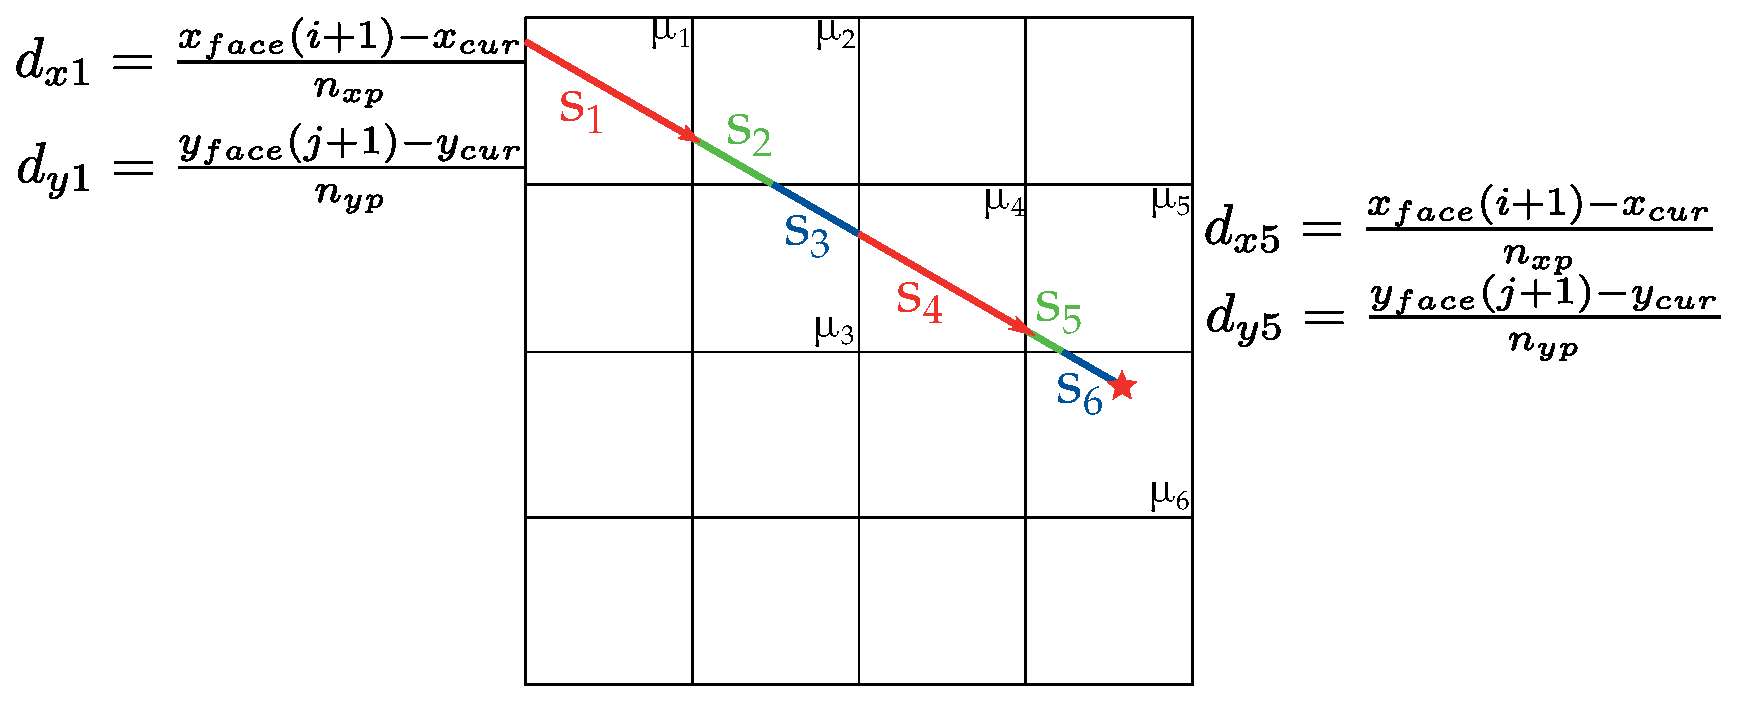
\includegraphics[width=0.75\textwidth]{grid_explain.eps}
	\caption{Illustration of photon propagation through a 2D grid. $d_{x1}$, and $d_{y1}$ are the distances to the voxel walls in the x and y directions in the $\mu_1$ voxel. In this case $S_1=d_{x1}$ as $d_{x1}$ is smaller than $d_{y1}$, thus the photon hits the voxel wall in the $x$ direction. For the $\mu_5$ voxel, $d_y$ is smaller, thus the photon hits the voxel wall in the $y^{th}$ direction.}
	\label{fig:voxelpropexplain}
\end{figure}

This whole process is repeated until the photon undergoes an interaction event or leaves the voxel medium.
The next step in the algorithm is the interaction event, which can consist of either: scattering, absorbing or another microphysics phenomena. 

\subsubsection*{Photon Interaction Event}\label{sec:photscatterabsorb}

The next section of the algorithm is to decide how the photon interacts with the medium, either via scattering or absorption. There are other interaction events that can occur, however descriptions of these are left for the chapters that detail these behaviours.
\medskip

To decide whether a packet scatters or absorbs involves generating a random number, $\xi$, and comparing it against the albedo, $a$. 
If $\xi < a$ then the packet scatters, otherwise it is absorbed. 
% The random number is compared to the albedo, and if the random number is less than the albedo then the packet scatters, otherwise the packet is absorbed.

\paragraph{Packet Absorption}\hspace{0pt}\\
\\
If the interaction event is a photon packet absorption, then the algorithm terminates the photon packets and starts the next photon packet, see~\nameref{sec:terminator}.

\paragraph{Packet Scattering}\hspace{0pt}\\
\\
If the interaction event is a packet scattering, then the packet is scattered into a new direction and the above processes are carried out until a termination clause is met, see~\nameref{sec:terminator}.

Depending on the medium being simulated, it can either be isotropic or anisotropic scattering. 
For the isotropic case, new $cos\left(\theta\right)$ and $\phi$ angles are sampled uniformly, and the direction vectors set as in section~\nameref{sec:photlaunch}.
For the case where the scattering is anisotropic the calculation of the scattering angles, $\theta$ and $\phi$, is more complicated.
The random sampling of the scattering angles, $\theta$ and $\phi$, are valid in the ``centre of mass'' frame containing the scatter, incident and scattered ray.
The photons position is updated in the lab frame, thus the direction vectors also have to be updated in the lab frame.
This means that the scattering angles need to be rotated into the lab frame.
For the isotropic case assume that the scattering is also isotropic in the lab frame, thus the new direction vector is easily calculated.
However this is not the case for anisotropic scattering, as the centre of mass frame has to be rotated into the lab frame.

\medskip

\Cref{fig:labframerotate} and~\cref{eqn:scatrotate} show how this process is achieved.
Where $\mathbf{n}=(n_x,n_y,n_z)$, $\mathbf{n_s}=(n_{x}^{new},n_{y}^{new},n_{z}^{new})$, $\theta_s$ is chosen from the phase function~\cref{eqn:henyeysample}, and $\varphi_s=2\pi \xi$ with $\xi$ being a random number in the range 0 to 1.
\begin{equation}
	\begin{aligned}
		n_{x}^{new} &= \frac{sin\theta_s}{sin\theta} \left(n_x\ n_y\ cos\varphi_s - n_y\ sin\phi_s\right) + n_x\ cos\theta_s \\
		n_{y}^{new} &= \frac{sin\theta_s}{sin\theta} \left(n_y\ n_z\ cos\varphi_s + n_x\ sin\phi_s\right) + n_y\ cos\theta_s \\
		n_{z}^{new} &= -sin\theta_s\ cos\varphi_s + n_z\ cos\theta_s
	\end{aligned}
	\label{eqn:scatrotate}
\end{equation}

\begin{equation}
cos\theta_s = \frac{1+g^2-\left(\frac{1-g^2}{(1-g+2g\xi)^{3/2}}\right)^2}{2g}
\label{eqn:henyeysample}
\end{equation}


\begin{figure}[!ht]
	\centering
	\includegraphics[width=0.5\textwidth]{frame-rot.pdf}
	\caption{Illustration of rotating the centre of mass frame to the lab frame. $\mathbf{n}$ is the direction vector of the photon before scattering, and $\mathbf{n_s}$ is the scattered direction vector. $\theta$ and $\varphi$ are the scattering angles. $z_s$ is in the same direction as $\mathbf{n}$.}
	\label{fig:labframerotate}
\end{figure}


\subsubsection*{Termination}\label{sec:terminator}

The final section of the \gls*{mcrt} algorithm is to check if tit should be terminated. This is a simple check to see if there are any more photons to run.
If there are more photons to run then the algorithm goes back to the~\nameref{sec:photlaunch} section and continues from there.
If there are no more photons the algorithm terminates and any results are written out.


\subsubsection*{Scored Quantities}\label{sec:fluencecalc}

As~\gls*{mcrt} is a computational method, a wealth of information is able to be recorded during the simulation.
From the paths of individual photons, to average scattering angles and more.
However it is not practical to record all this information for every simulation, as this would lead to inefficient simulations, and expensive data storage solutions.
Thus for a given problem only the pertinent information is stored.

One important recorded variable is fluence.
Fluence is the number of photons entering a sphere per unit cross section area~\cite{rogers1990monte}.
In practise the average fluence per area is used,~\cref{eqn:jmean}, as this is easier to calculate in an~\gls*{mcrt} code.
Lucy showed that the average fluence per area is proportional to the sum of the path length through a volume~\cite{lucy1999computing}:

\begin{equation}
J_i = \frac{L}{NV_{\varsigma}}\sum l 
\label{eqn:jmean}
\end{equation}

\noindent Where:

\indent $J_i$ is the mean intensity such that the fluence is $\Phi=4\pi J$ [$W\ m^{-2}$];

\indent $L$ is the luminosity or power of the light source [$W$];

\indent $N$ is the total number of photon packets [-];

\indent $V_{\varsigma}$ is the volume of the $\varsigma^{th}$ voxel [$m^3$];

\indent and $l$ is the path length of a photon packet through the $\varsigma^{th}$ voxel [$m$]. 

\medskip

The majority of the chapters in the thesis make use of~\cref{eqn:jmean} or modified versions of it as the main scored quantity, e.g. to determine absorbed energy.

Other common scored quantities are the exit location of a photon, the wavelength of an exiting photon or the distribution of photon packet absorption.

\subsection{Code Details}

This section describes the implementation of the \gls*{MRCT} code and a description of  parallelisation.

\subsubsection*{Code}

All code in this thesis is written in modern Fortran\footnote{modern Fortran is considered anything past Fortran 95~\cite{metcalf2011modern}.}.
All subroutines and functions are contained in modules (with the exception of the main program---main.f90).
This is done in order to be able to ``hide'' data from subroutines and functions, and to arrange the code that relates to other parts of the code in the same file.
Having the code in modules also allows the use of runtime allocation of memory for arrays.
This enables the user to specify the size of arrays depending on the need of the user for the problem at hand.

Modules are classified into three different types: data, routines and dependencies.
Data modules are modules that contain no function or routines, but store variables that can be accessed anywhere in the program when required.
Routine modules contain the subroutines and functions used in the code.
Finally dependency modules are the modules that have not been written by me, and thus the code depends upon them in order to run.

\Cref{fig:codegraph} show the relationship between the various modules, for a basic version of the \gls*{mcrt} as described in~\nameref{sec:algorithmMCRT}.

\medskip
\indent Using~\cref{fig:codegraph} as a reference each module contains:

\noindent {\color{green}\textit{mcpolar.f90}} is the entry point of the code. It calls all other subroutines and functions, as well as setting up various variables and printing progress.

\noindent {\color{lightblue2}\textit{ch_opt}} is the module where the optical properties are set or changed.

\noindent {\color{lightblue2}\textit{gridset_mod}} is where the optical properties grid and voxel walls are set.

\noindent {\color{lightblue2}\textit{subs}} contains general purpose routines that are used in various different parts of the code.

\noindent {\color{lightblue2}\textit{writer_mod}} contains routines that write out the results of the simulation.

\noindent {\color{lightblue2}\textit{inttau2}} is the module that contains the routines that propagate the photon through the voxel grid.

\noindent {\color{lightblue2}\textit{sourcph_mod}} contains the routines that initialise the photon position and direction.

\noindent {\color{lightblue2}\textit{stokes_mod}} contains the routine that calculates the scattering direction after a scattering event.

\noindent {\color{red}\textit{iarray}} is a data module that contains all the arrays in the code.

\noindent {\color{red}\textit{constants}} is a data module that contains all the constants and filepaths needed in the code.

\noindent {\color{gray}\textit{ieee_arithmetic}} is an external dependency that gives various arithmetic checking routines such as is_nan().

\noindent {\color{lightblue2}\textit{vector_class}} is a module that contains the vector type, and all its associated operations such as cross and dot products of vectors.

\noindent {\color{red}\textit{photon_vars}} is a data module that contains the data pertaining to each photon, such as wave length or energy.

\noindent Finally, {\color{red} \textit{opt_prop}} contains the data about the current optical properties such as the albedo, and absorption coefficient.


\begin{figure}[!ht]
	\centering
	\includegraphics[width=0.95\textwidth]{graph-code.pdf}
	\caption{Source code hierarchy, showing the relationship between different modules. Green is the entry point for the simulation. Red are the data modules, light blue are the routine modules, and grey are the external dependencies.}
	\label{fig:codegraph}
\end{figure}



\subsection*{Parallelisation of the MCRT Algorithm}\label{sec:parasec}

As mentioned in the previous sections, \gls*{mcrt} can be computationally intensive, especially when dealing with highly scattering mediums. Fluorescence can also cause simulations times to drastically increase as photons are no longer ``killed'' off, but rather re-emitted at a new wavelength. Other optical processes such as Raman scattering are highly unlikely events, which again can lead to a dramatic increase in simulation times, as many photons are required to be simulated in order to get ``good'' statistics.

Fortunately \gls*{mcrt} is classed as an ``embarrassingly parallel'' problem\footnote{However this is not true for all \gls*{mcrt} applications. For example, using the Bjorkman $\&$ Wood~\cite{bjorkman2001radiative} immediate temperature corrections method, turns \gls*{mcrt} into a different class of parallel problem~\cite{robitaille2011hyperion}.}.
This means that it is trivial to parallelise in comparison to other algorithms. 
The reason that \gls*{mcrt} is classed as ``embarrassingly parallel'', is that the algorithm can be split up onto separate processors, with little need for communication between them. 
In reality this means that $n$ copies of the algorithm can run on $n$ cores in a processor, with communication taking place at the start and end of each simulation run. 

All the code in this thesis is parallelised using \gls*{mpi}~\cite{gropp2014using,gropp2014usingadv}, with the only communication taking place at the end, where the results are collated on to all processes.
The one exception to this is in~\cref{chap:ablation}, where the heat diffusion calculation needs communication between the processes during the calculation.

The parallel efficiency of a code depends on the problem, and the number of photon packets run.
To determine the speedup of a given problem Amdahl's law is used~\cite{amdahl1967validity}:

\begin{equation}
speedup = \frac{1}{(1-P)+P/N}
\end{equation}

Where $P$ is the fraction of the code that is parallel, and N is the number of cores the code is run on.
The consequence of Amdahl's law is as $N$ tends to infinity the speedup tends to a maximum:

\begin{equation}
speedup_{max}=\frac{1}{1-P}
\end{equation}

The value of P varies from problem to problem, and the number of photon packets run.
\Cref{fig:paratest} shows the results of the profiling of the code, for various numbers of cores.
This test consisted of running the same number of photons, in a highly scattering medium of size $2~cm^3$.
This yielded a $P$ of $0.999010 \pm 0.000045$, and a maximum speedup of 1010.1.


\begin{figure}[!ht]
	\centering
	\includegraphics[width=0.75\textwidth]{profile-mcrt.pdf}
	\caption{Performance of the parallelisation of the MCRT code using MPI.}
	\label{fig:paratest}
\end{figure}


There are other ways the code could be parallelised, including task farms and domain decomposition~\cite{barney2010introduction}.
However these methods are more involved to set up and validate, so the simplest approach was taken.
\FloatBarrier
\section{Validation of MCRT Code}\label{sec:validation}

As the Monte Carlo method is an algorithm that depends upon random numbers, it is sometimes hard to ensure the correct result is obtained.
Or to put it another way:
\medskip

``Monte Carlo is easy to do wrong!'' G.W. Collins III~\cite{bjormaneasymonte}

\medskip

Thus the code has to be validated against various theoretical/experimental and other simulations, to determine whether the results are correct.

The main benchmark of the~\gls*{mcrt} code, is a comparison against an expression for fluence as a function of depth~\cite{gardner1993fluorescence}.
This expression has also been fitted to by other~\gls*{mcrt} simulations~\cite{jacques1993photobleaching}.

\begin{equation}
\Psi(z)=\Psi_0(C_1e^{-k_1z/\delta}-C_2e^{-k_2z/\delta})
\label{eqn:jacqmatch}
\end{equation}

\noindent Where:

\indent $\Psi(z)$ is the penetration of the excitation light, or equivalently the fluence rate [$W\ cm^{-2}$];

\indent $\Psi_0$ is a normalisation constant [$W\ cm^{-2}$];

\indent $C_n$ and $k_n$ are fitted coefficients [-];

\indent and $\delta$ is the optical penetration depth, defined as $\delta=1/\sqrt{3\mu_a(\mu_a+\mu_s(1-g))}$, [$cm$].

\medskip

Jacques \textit{et al.}, in their simulation used two different wavelengths, 420~nm and 630~nm.
The medium in the simulation is a infinitely wide slab with a depth of 1~cm, with uniform optical properties. 
The medium has a refractive index of 1.38.
The $g$ value is in the range 0.7 -- 0.9, and the optical properties are as in~\cref{tab:jacqprops}.

\begin{table}[!ht]
\begin{tabular}{llllllll}
                                   & \multicolumn{1}{c}{{\ul Absorption}} & \multicolumn{1}{c}{{\ul Scattering}}    & \multicolumn{4}{c}{{\ul Penetration}}          &             \\
\multicolumn{1}{l|}{Wavelength/nm} & \multicolumn{1}{l|}{$\mu_a$/$cm^{-1}$} & \multicolumn{1}{l|}{$\mu_s(1-g)/cm^{-1}$} & C1   & k1   & C2   & \multicolumn{1}{l|}{k2}   & $\delta/cm$ \\ \hline
\multicolumn{1}{l|}{420}           & \multicolumn{1}{l|}{1.8}             & \multicolumn{1}{l|}{82}                 & 5.76 & 1.00 & 1.31 & \multicolumn{1}{l|}{10.2} & 0.047       \\
\multicolumn{1}{l|}{630}           & \multicolumn{1}{l|}{0.23}            & \multicolumn{1}{l|}{21}                 & 6.27 & 1.00 & 1.18 & \multicolumn{1}{l|}{14.4} & 0.261      
\end{tabular}
\caption{Table of optical properties and determined coefficients from Jacques \textit{et al.}~\cite{jacques1993photobleaching}.}
\label{tab:jacqprops}
\end{table}

Using these values Jacques \textit{et al.} calculated values for $C_1,\ C_2,\ k_1$ and $k_2$ using their \gls*{mcrt} code.
The above optical properties and medium dimensions\footnote{The infinitely wide slab is implemented so that when a photon leaves the one of the sides of the voxel grid, it is moved to the other side of the grid, retaining its original direction vectors.} are recreated in the code and a value of 0.9 was chosen for $g$.
8 million photons were run for the simulation.
This yielded the result as in~\cref{fig:matchjacq}.

\begin{figure}[!ht]
	\centering
	\includegraphics[width=0.95\textwidth]{validation-jacques.pdf}
	\caption{Figure shows the fluence as a function of depth. Figure also shows comparison to the Jacques MCRT simulation and the MCRT as described in this chapter.}
	\label{fig:matchjacq}
\end{figure}


Fitting~\cref{eqn:jacqmatch} to the data calculated by our~\gls*{mcrt} code for $630~nm$, gave: $C_1 = 6.425$, $C_2=1.083$, $k_1=1.0$, and $k_2=12.966$.
For $420~nm$ gave: $C_1 = 5.600$, $C_2=0.838$, $k_1=1.003$, and $k_2=9.846$.
These are in good agreement (with in code differences) with Jacques \textit{et al.} results.

\section{Conclusion}

The Monte Carlo method relies on generating random numbers in order to calculate unknown variables in problems.
The Monte Carlo method can be used to calculate radiation transport in order to numerically solve the~\gls*{rte}.
\Gls*{mcrt} is the most flexible of the methods available to solve the~\gls*{rte}, allowing arbitrary geometries, light sources and turbid media.
\Gls*{mcrt} also allows the inclusion of various microphysics such as polarisation, Raman scattering and fluorescence.
However the~\gls*{mcrt} method does have the downside, that for some problems, many photon packets must be run in order to achieve a good signal to noise ratio.
Though this is becoming less of an issue due to increased computational available capacity and~\gls*{mcrt} being classed as an ``embarrassingly parallel'' problem, allowing it to be easily parallelised.

The MCRT algorithm as described in this chapter forms the basis for this thesis.
Each subsequent chapter builds upon the algorithm in order to solve new problems.
\chapter{Computational modelling of tissue ablation}



%More background on why developing the laser ablation model. 
%What is the medical reason to want this. 
%What medical procedures are done with laser ablation? 
%What are the outstanding issues/questions that your model can be used to answer? mention pig skin

%Details of laser pulsing. now add this in experimental results section
%Time steps, convergence tests, etc
%Time for holes to be drilled by laser.
%Low intensity damage
%in equation 9, could A and Delta-E be functions of temperature?

\section{Introduction and background}

Lasers are used in wide variety of medical procedures not limited to: coagulating scalpels, port wine stain removal, tattoo removal, hair removal, and skin rejuvenation~\cite{amini2010ultrafast, tan1989treatment,kuperman2001laser,liew2002laser,hardaway2002nonablative}.
One class of laser used in these procedures are ablative lasers. Ablative lasers are usually high powered lasers targeted at a specific chromophore in the skin, to partially or fully remove layers of skin. These types of lasers are commonly used for aesthetic procedures such as: skin rejuvenation~\cite{hardaway2002nonablative}, and removal of various diseases such as Rhinophyma~\cite{shapshay1980removal} or lesions/nodules~\cite{valcavi2010percutaneous}. They have also recently been investigated as a means of better drug delivery in the skin for photo-dynamic therapy (PDT) treatments~\cite{haedersdal2010fractional}.\\

One downside to using lasers to remove tissue, it that unlike a scalpel, where the surgeon has full control of the depth of the incision, ablative lasers are not as predictable. Lasers can also cause  unwanted thermal damage to the surrounding areas, leading to unwanted effects.
Ablative lasers, and fractionated ablative lasers (ablative lasers where the power is spread over several beams, such as to leave viable tissue around zones of damaged/necrotic tissue~\cite{manstein2004fractional}). Currently the only reliable method to measure the depth of the ablative holes, is via a biopsy, which is an invasive procedure. We propose to use optical coherence tomography (OCT) to measure the ablative crater non-invasively \textit{in-vivo}. The OCT measurements are then backed up by a computational model. This computational model could then be used to predict the depth of the ablative crater when using a certain power for various different applications such as: laser assisted drug delivery, and various cosmetic applications.

This chapter examines using Monte Carlo radiation transport techniques coupled to a heat transfer simulation, in order to study the thermal damage to tissue due to fractional lasers. We present experimental work carried out by our collaborators at the University of Dundee and the photobiology department at Ninewells hospital. This experimental work was carried out on porcine tissue, using CO$_2$ and Er:YAG lasers.

\section{Methods}

In order to replicate the experimental work \textit{in silica}, our numerical model has three main portions. The first is the Monte Carlo radiation transport method (MCRT) that models light transport through tissue so that we can calculate the laser energy deposited as a function of time and space. The second, a finite difference method (FDM) which is used to calculate the heat diffusion within the tissue due to the absorbed laser energy. Finally, a tissue damage model to track the damage to the tissue caused by the laser. All these individual portions are connected together to create our numerical model. Each portion of the numerical model is described below in more detail.

\subsection{Monte Carlo radiation transport (MCRT)}

MCRT is the `gold standard' for simulating the transport of light through biological tissue *ref*. It uses interaction probabilities and random numbers in order to model the `random walk' that photons undergo in a turbid medium. These `packets' can undergo go scattering, absorption and various other physical process \cite{yao1999monte,welch1997propagation}. MCRT has been used to model light-tissue interactions in many different medical and biophotonic applications \cite{campbell2015monte}*more refs*. MCRT is used here to calculate the energy deposited by the laser, which is then passed to the heat transport simulation.\\

The tissue medium for the MCRT and heat transport simulations is a 3D voxel model (\cref{fig:voxel-model}). This allows the variation of optical and thermal properties from voxel to voxel, making it the ideal type of grid for modelling tissue ablation. We use  n x n x n voxels *still changing this*, representing a tissue sample size of 1.1 $\times$ 1.1 $\times$ 0.5 cm. We assume the porcine skin is uniform, so that initially our voxel model is uniform, and the optical properties of porcine skin at the wavelength of interest is that of water, see \cref{fig:waterabsor}.\\


\begin{figure}
\centering
\includegraphics[scale=0.25]{./ablation/images/voxel-model-render.png}
\caption{Example of a possible voxel model, with three different layers, various holes due to ablative pixel beam lasers. Each voxel represents a different optical/thermal propertty of the tissue medium.}\label{fig:voxel-model}
\end{figure}

The original MCRT code was developed for astronomy applications \cite{wood1999model,wood2005estimating}, and has since been adapted for medical applications~\cite{campbell2015monte,barnard2018quantifying}.

\Cref{fig:algo}. shows the overall algorithm for the simulation, including the MCRT portion. 
The MCRT portion of the algorithm begins with determining where the photon enters the medium. This is calculated by randomly selecting one of the pixel beams, from the 9x9 array of pixel beams. Next the position on the surface of the medium is calculated. As the profile of the pixel beams are unknown, they are assumed to be uniformly circular *maybe change to gaussian??*. Thus, the packets position is uniformly sampled on a circle the width of the pixel beam.

Once the packet enters the simulation, a propagation distance for the packets is calculated using \cref{eqn:propdist}. The packet then moves this distance before undergoing an interaction event. This can be either scattering or absorption. This process is repeated until the photon has either been absorbed or exits the medium.

\begin{equation}
L = -\tfrac{ln(\xi)}{\mu_a}
\label{eqn:propdist}
\end{equation}

\noindent Where:\\
\indent $\xi$ a random number ($\tau = -ln(\xi)$, $\tau$ is the optical depth);\\
\indent $\mu_a$ is the absorption coefficient;\\
\indent L is the physical distance.\\

\Cref{eqn:propdist} is the equation for a uniform medium. As the medium we are simulating changes over time due to thermal damage this equation has to be adapted for a 3D Cartesian grid. Each voxel 
can have different optical properties, thus the photon packet is moved on a voxel by voxel basis. To start the movement process, a random number is generated, which is used to sample an optical depth the photon packet will travel. Next the photon enters the voxel and the maximum distance the photon can travel in the new voxel is calculated along the photons trajectory. If this optical distance is less than the optical depth sampled, then the photon enters the next voxel. If the distance is larger than the sampled optical distance then the photon has an interaction event in that voxel. The photon packet moves to the interaction event in the voxel and then undergoes scattering or absorption. The whole process is repeated until the photon `dies' via absorption or leaving the medium.

This in turn is again repeated for all the photons, until all the photons have been absorbed or have escaped the tissue medium. We use 5 million photons per MCRT simulation run.\\

\begin{figure}
\centering
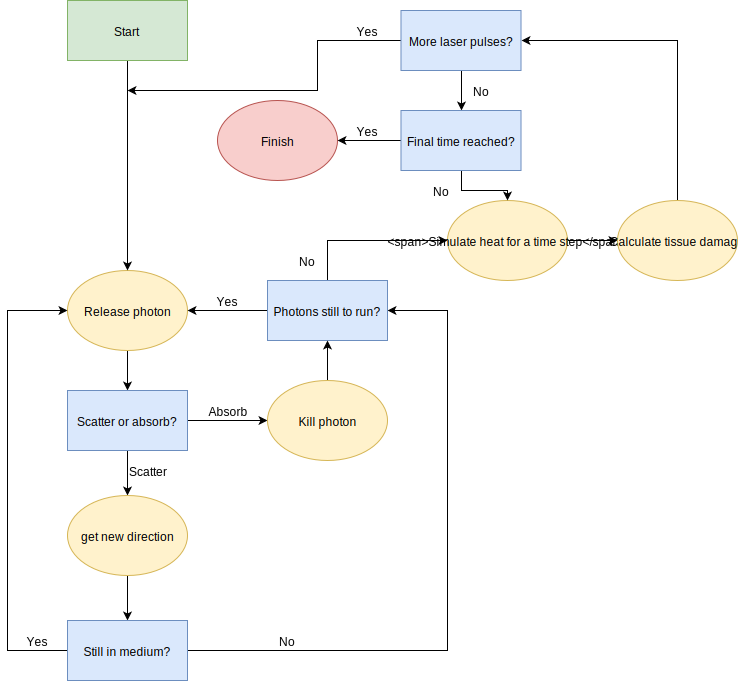
\includegraphics[scale=0.5]{./ablation/images/flowchart.pdf}
\caption{Flowchart of the tissue ablation algorithm.}
\label{fig:algo}
\end{figure}

We calculate the absorbed energy using the path length counter method devised by Lucy \cite{lucy1999computing}. The energy absorbed per voxel is calculated as:

\begin{equation}
E_{i}^{abs} = \frac{L}{N \Delta V_i}\sum\mu_a s
\label{eqn:Eabs}
\end{equation}

\noindent Where:\\ 
	\indent L is luminosity [$W$];\\
	\indent N is the number of photons;\\
	\indent $\Delta V_i$ is the volume of the $i^{th}$ voxel [$m^{-3}$];\\
	\indent $\mu_{a,i}$ is the absorption coefficient of the $i^{th}$ voxel [$cm^{-1}$];\\
	\indent and s is the pathlength of a photon packet through the $i^{th}$ voxel [$cm$].\\
	
\begin{figure}
\centering
\includegraphics[scale=0.25]{./ablation/images/jmea-explain.png}
\caption{Red lines are photon paths within a voxel. Black lines photon paths outwith the voxel. Red photon paths are summed up in order to calculate the absorbed energy within each voxel.}
\label{fig:jmea-explain}
\end{figure}	
		
This grid of absorbed energy is then passed to the heat transport portion of the simulation.

\subsection{Heat transport}

In order to model the transport of heat in porcine skin, we use the standard parabolic heat equation:

\begin{equation}
\rho c_p \frac{\partial T}{\partial t}= \nabla \cdot (\kappa \nabla T) + \dot{q}
\label{eqn:heat}
\end{equation}

\noindent Where:\\
	\indent $T(x, y, z, t)$ is the temperature as a function of time and space [\textit{K}];\\
	\indent $\kappa$ is the thermal conductivity [$W\cdot m^{-1}\cdot K^{-1}$];\\ 
	\indent $\rho$ is the density [$Kg \cdot m^{-3}$];\\
	\indent $c_p$ the specific heat capacity [$J\cdot K^{-1}$];\\
	\indent $\dot{q}(x,y,z,t)$ is the source/sink term as a function of time and space [$W\cdot m^{-3}$].\\
	
We assume that $\kappa$	is constant during heat transport and only changes between heat transport and MCRT portions of the simulation (see Section Tissue damage), thus:

\begin{equation}
\frac{\partial T}{\partial t}= \alpha \nabla^2 T + \dot{q}
\label{eqn:heatreal}
\end{equation}
	
Where $\alpha = \tfrac{\kappa}{\rho c_p}$ is the thermal diffusivity [$m^2 s^-{1}$]	\\
	
The $\dot{q}$ term is a heat source/sink term. The heat source in this simulation is due to the laser, and we assume the only loss of heat to the surrounding medium is via convection and conduction.
	
These boundary conditions must be considered. All faces of the cube, bar the laser facing face, are considered to be pinned at 5$^{\circ}$C, as the porcine skin was kept cooled prior to experimental work. The laser facing face has a simple convective BC:	

\begin{equation}
\dot{q}_c = -hA(T - T_\infty)
\label{eqn:bceqns}
\end{equation}

\noindent Where:\\
	\indent \textit{h} is the heat transfer coefficient [$W m^{-2} K$];\\
	\indent and \textit{A} is the area of the grid element, that is radiating/convicting heat away [$m^-{2}$].\\

As \cref{eqn:heatreal} is generally hard to solve in arbitrary geometries with complex boundary conditions we employ a numerical method to solve \cref{eqn:heatreal}.
The numerical method we employ in order to solve \cref{eqn:heat} is a the finite difference method (FDM)\cite{ozisik1994finite}. FDM is derived from the Taylor series approximation for derivatives. A function $f(x)$ is discretised onto a grid with \textit{N} nodes (see~\cref{fig:fdmexplain}). Then at node \textit{i} we can use the Taylor series approximation in the forward ($+\text{ive}\ x$ direction) and backward ($-\text{ive}\ x$ direction), and combine the 1$^{st}$ and 2$^{nd}$ derivatives in 1D, where: \textit{i} is the grid point at $x_o$, $i$+1 is the point at $x_0+\Delta x$, and \textit{i}-1 is the grid point at $x_{o}-\Delta x$.

\begin{figure}
  \vspace{-10pt}
  \begin{center}
    \includegraphics[width=0.48\textwidth]{./ablation/images/fdm.pdf}
  \end{center}
  \caption{Finite difference methods discretisation of \text{f(x).}}\label{fig:fdmexplain}
    \vspace{-20pt}
\end{figure}

\begin{subequations}
\begin{align}
\frac{df}{dx} &= \frac{f_{i+1} - f_{i}}{\Delta x}  &(forward)\\
\frac{df}{dx} &= \frac{f_{i} - f_{i-1}}{\Delta x}  &(backward)\\
\frac{df}{dx} &= \frac{f_{i+1} - f_{i-1}}{2\Delta x}  &(central)\\
\frac{d^2f}{dx^2} &= \frac{f_{i-1}-2f_i+f_{i+1}}{\Delta x^2} &(central)
\end{align}
\end{subequations}


Thus \cref{eqn:heatreal}, in 1D, becomes:

\begin{equation}
T_{i+1}^{n+1} =  \Delta t\alpha \frac{T_{i-1}^n-2T_i^n+T_{i+1}^n}{\Delta x^2} + T_i^n + \dot{q}
\label{eqn:simplefdm}
\end{equation}

\begin{figure}
  \begin{center}
    \includegraphics[width=0.48\textwidth]{./ablation/images/fdm-stencil.pdf}
  \end{center}
  \caption{Finite difference method stencil for simple explicit scheme}\label{fig:fdmstencil}
    \vspace{-20pt}
\end{figure}

\Cref{eqn:simplefdm} is called the `simple explicit form of finite-difference approximation'\cite{ozisik1994finite}. \Cref{fig:fdmstencil} shows the `stencil' of this scheme, where there are three known points at time \textit{N}, and just one unknown at time \textit{N+1}. We use a simple explicit scheme here, due to its ease of implementation. This yields for the more general 3D case:


\begin{align}
U_{xx} &= \frac{\alpha}{\Delta x^2} (T^N_{i-1,j,k} - 2T^N_{i,j,k} + T^N_{i+1,j,k}) \label{eqn:FDMheat1}\\
U_{yy} &= \frac{\alpha}{\Delta y^2} (T^N_{i,j-1,k} - 2T^N_{i,j,k} + T^N_{i,j+1,k}) \label{eqn:FDMheat2}\\
U_{zz} &= \frac{\alpha}{\Delta z^2} (T^N_{i,j,k-1} - 2T^N_{i,j,k} + T^N_{i,j,k+1}) \label{eqn:FDMheat3}\\
T^{N+1}_{i,j,k} &= \Delta t\ (U_{xx} + U_{yy} + U_{zz}) + T^{N}_{i,j,k} + \tfrac{\alpha \Delta t}{\kappa}\dot{q_L} \label{eqn:FDMheat4}
\end{align}

\noindent Where:\\
	\indent $T^{N+1}_{i,j,k}$ is the new temperature at node $i,j,k$ [$K$];\\
	\indent $T^N_{i,j,k}$ is the temperature at node $i,j,k$ at the current time step [$K$];\\
	\indent $\alpha$ is the thermal diffusivity [$m^2\cdot s^{-1}$];\\
	\indent $\kappa$ is the thermal conductivity [$W/m\cdot K$];\\
	\indent $\Delta x\ etc.$ is the size of the grid element in the $p^{th}$ direction [$m$].\\

Incorporating B.Cs on the top air exposed face:

\begin{equation}
U_{zz} = \tfrac{\alpha}{\Delta z^2} (\tfrac{2 \Delta z}{\kappa} (-h(T^N_{i,j,k}-T^N_\infty) ) -2 T^N_{i,j,k} + 2T^N_{i,j,k+1}) 
\end{equation}

As the lasers *maybe remove s?* operate in a pulsed mode, we account for this in our simulation. We assume that the pulse shape is a top-hat pulse for simplicity. In the heat simulation we have an additional variable in the term $laserOn\cdot\tfrac{\alpha \Delta t}{\kappa}\dot{q_L}$ in \cref{eqn:FDMheat4}. This addiational variable, laserOn, is a boolean value, which is defined as:

\[   
laserOn = 
     \begin{cases}
       \text{1,} &\quad\text{if time}\le\text{pulse length}\\
       \text{0,} &\quad\text{if time}>\text{pulse length}.\\
     \end{cases}
\]

In the instance where there is more than one pulse, the laser is turned on and off based upon the pulse frequency.\\

As we are using a simple explicit FDM, the time step is constrained in order to make the solution stable. For a cubic 3D FDM without prescribed flux BCs, yields the constraint: $\Delta t \leq \tfrac{\alpha \Delta x^2}{2\beta}$. However as we have a flux prescribed boundary condition, the constraint on the time is more severe. Along with this time restraint, the pulse length of the laser also has to be considered. If the time step of the heat simulation is too large it will not account for the heat deposited by the laser. Thus, the timestep has to be an order of magnitude smaller than the shortest laser pulse.

As the timestep is small, and the grid resolution large, the resultant simulation is slow. Thus the code has been fully parallelised to improve performance. Both the MCRT and heat simulation are independently parallelised. As discussed in \cref{sec:mcrt-para}, the MCRT simulation is fully parallelised, and the results are passed to the heat simulation.

Parallelisation of the heat simulation is more involved than the `embarrassingly parallel' class of problems that MCRT belongs to. This is due to the heat simulation needing to know the temperature of adjacent nodes. Thus information will have to be passed from each individual core during computation, as opposed to doing the information passing at the end of the simulation \textit{\`a la} MCRT parallelisation.\\
The heat simulation is parallelised using a technique called `halo swapping'. This involves splitting up the computational domain (see \cref{fig:griddecomp}), in this case the tissue medium, and doing the calculations on each domain on a separate core. The `halo swapping' comes in when cores need to communicate with each other about updating their boundary temperature nodes (see \cref{fig:haloswap}).\\

On a workstation computer these simulations were carried out on (Intel Xeon E3-1245 v5, 8 core @3.5GHz) led to a speed up of $\sim$6, over the serial simulation. Using Amdahl's law\cite{amdahl1967validity}, the serial portion of the simulation is $\sim$ 5\%, giving a theoretical speed up $\sim$ 20 times the serial simulation.


\begin{figure}
\vspace{-45pt}
\centering
\includegraphics[scale=.35]{./ablation/images/grid-decomp.pdf}
\caption{Computational domain decomposition. Total computational domain is evenly divided between cores in the CPU. This is done via layers of the domain in the z direction. Information is passed to/from cores via the `halo swap' process (see~\cref{fig:haloswap}).}
\label{fig:griddecomp}
\vspace{-10pt}
\end{figure}

\begin{figure}
\centering
\def\svgwidth{350pt}
\input{./ablation/images/halo.pdf_tex}
\caption{Halo swapping. Process A updates the area in red and blue on the left. It updates the blue area which is sent to process B as B's `halo'. Process B cannot update it's own halo, but rather updates the halo for process A.}
\label{fig:haloswap}
\end{figure}


After the heat transport has been completed, the grid of temperatures is passed to the tissue damage portion of the simulation.
\newpage
\subsubsection{Validation of heat transport numerical method}

In order to validate the numerical method we employ to solve the heat equation, we compare the numerical method against an easily solvable case. We solve the heat equation on a cube, side L, in a surrounding medium of 0$^{\circ}$C. The cube is initially at temperature 37$^{\circ}$C and we calculate the temperature at time \textit{t=*input here*s}. Thus the boundary conditions are:\\

\begin{align}
T(0,y,z,t)&=T(x,0,z,t)=T(x,y,0,t)=0^{\circ}\text{C} \label{eqn:bc1}\\
T(L,y,z,t)&=T(x,L,z,t)=T(x,y,L,t)=0^{\circ}\text{C} \label{eqn:bc2}\\
\end{align}

The thermal diffusivity~($\alpha$)=, which corresponds to that of water *ref*.\\


Assuming a separable solution in Cartesian coordinates for the heat equation yields:
\begin{equation}
\begin{split}
T(x,y,z,t)=&(A_1Cos(\alpha x) + A_1Sin(\alpha x))\cdot\\
&(B_1Cos(\beta y) + B_1Sin(\beta y))\cdot\\
&(C_1Cos(\gamma z) + C_1Sin(\gamma z))\cdot e^{-\alpha\mu^2t}\\
\end{split} 
\end{equation}

\begin{equation}
\mu^2=\alpha^2+\beta^2+\gamma^2
\end{equation}

Applying the boundary conditions (\cref{eqn:bc1,eqn:bc2}) gives:

\begin{equation}
A_1=B_1=C_1=0\
\text{and}\ \alpha=\frac{\pi n}{L}\ \beta=\frac{\pi m}{L}\ \gamma=\frac{\pi p}{L}
\end{equation}

\begin{equation}
\therefore  T_{nmp}(x,y,z,t)=A_{nmp}Sin\left(\frac{\pi n x}{L}\right)\cdot Sin\left(\frac{\pi m y}{L}\right)\cdot Sin\left(\frac{\pi p z}{L}\right)
\end{equation}

This yields the following solution for the heat equation using the principle of superposition:

\begin{equation}
T(x,y,z,t)=\sum^\infty_{n=1,3,..}\sum^\infty_{m=1,3,..}\sum^\infty_{p=1,3,..}\frac{2368}{\pi^3nmp}Sin(\frac{\pi n x}{L})Sin(\frac{\pi m y}{L})Sin(\frac{\pi p z}{L})e^{(-\lambda^2t)}
\end{equation}

\noindent Where:\\
	\indent $\lambda^2=\alpha\pi^2(\tfrac{n^2}{L^2}+\tfrac{m^2}{L^2}+\tfrac{p^2}{L^2})$;\\
	\indent $n,m,p$ are odd integers;\\
	\indent and $L$ is the length of the cube.\\
	
At time, $t=*input*$s, a slice through the middle of the cube, $L=1~cm$,  yields \cref{fig:validation-heat}.

\begin{figure}	
\vspace{-10pt}
	\centering
	\includegraphics[width=\columnwidth]{./ablation/images/validation.pdf}
	\caption{Comparison between analytical solution and numerical method.}
	\label{fig:validation-heat}
	\vspace{-10pt}
\end{figure}	
	
	
\subsection{Tissue Damage}
\label{sec:tissuedamage}
The final portion of the simulation is the tissue damage model. We use the Arrhenius damage model, originally used as a kinetic model of reaction products in chemistry~\cite{pearce2009relationship}. It has since been adapted by various authors for modelling tissue damage \cite{hendriques1947studies,jiang2002effects}.

\begin{equation}
\Omega(t)=\int^{t_{f}}_{t_i} Ae^{(-\tfrac{\Delta E}{RT})}d\tau
\end{equation}


\noindent Where:\\
	\indent $\Omega$ is the damage value; \\
	\indent A is `frequency factor' [$s^{-1}$];\\
	\indent $\Delta E$ is activation energy [$J\cdot mol^{-1}$];\\
	\indent R is the universal gas constant [$J\cdot mol^{-1}\cdot K^{-1}$];\\
	\indent T is the temperature [$K$];\\
	\indent and $t_i$ and $t_f$ are the initial time and final time at $t_{crit}$.\\

It is reported that a value of $\Omega$ of 0.53, 1.0, and 10$^4$ relate to first, second, and third degree burns respectively~\cite{diller1983finite}. We use the Arrhenius damage model in order to better understand the amount of damage caused by the laser in the non-ablated areas of tissue. This can give us an insight into the various physical phenomena encountered in the OCT results.\\

We model tissue damage in three main sections: coagulated, dehydrated, and finally ablated sections.\\

Coagulated tissue is the the areas of the tissue where the temperature is above 43$^{\circ}$C, the threshold for damage but below 100$^{\circ}$C.
When areas of the tissue reach 100$^{\circ}$C water begins to boil off. This acts as a large heat sink for the absorbed laser energy, slowing down the rate of ablation. The ener

\begin{equation}
Q_{vapor}=laserOn\cdot\dot{q}\cdot \Delta t\cdot V_{i,j,k} + c\cdot M_{i,j,k}\cdot\Delta T
\end{equation}

\noindent Where:\\
	\indent $Q_{vapor}$ is the current energy in Joules that has been used to boil off the water in the voxel [$J$];\\
	\indent $laserOn$ is a boolean variable that determine if the laser is on or off [$-$];\\
	\indent $\dot{q}$ is the energy absorbed by the voxel due to the laser [$W\cdot m^{-3}$];\\
	\indent $\Delta t$ is the timestep [$s$];\\
	\indent $V_{i,j,k}$ is the volume of the $i^{th}$, $j^{th}$, $k^{th}$ voxel [$m^3$];\\
	\indent $c$ is the heat capacity of the voxel [$J\cdot K^{-1}$];\\
	\indent $M_{i,j,k}$ is the mass of the $i^{th}$, $j^{th}$, $k^{th}$ voxel [$Kg$];\\
	\indent and $\Delta T$ is the change in temperature the voxel would undergo, if the water was not boiling off.\\
	
As water boils off, the water content of each voxel changes. This affects the absorption coefficient, density, thermal conductivity, and heat capacity. Each of these vary linearly with water content per voxel\cite{choi2001analysis};

\begin{align}
W &= W_{init} - \left(W_{init} \cdot \left(\tfrac{Q_{current}}{Q_{vaporisation}}\right)\right) \\
\rho &= 6.16 \cdot 10^{-5}\ W + 9.38 \cdot 10^{-4} \\
c &= 2.5 \cdot 10^{3}\ W + 1.7\cdot 10^{3} \\
\kappa &= \rho \cdot 10^{-3} (0.454\ W + 0.174)
\end{align}

\noindent Where:\\
\indent $W$ is the water content (i.e W = 0.7 equates to 70\% water content);\\
\indent $W_{init}$ is the initial water content;\\
\indent $Q_{current}$ is the total energy absorbed by the $i^{th}$ voxel since the temperature reached 100$^{\circ}$C [$J$];\\
\indent $\kappa$ is the Thermal conductivity [$W\cdot m^{-1}\cdot K^{-1}$];\\
\indent and c is the heat capacity [$J\cdot Kg^{-1}\cdot K^{-1}$].\\

We define the ablation temperature ($T_a$) as occurring between 173 and 450$^{\circ}$C\cite{gerstmann1994char}. At the $T_a$ the tissue is removed and set the thermal and density properties to that of air.

The tissue structure is then fed back to the MCRT model and the whole process repeats until the average temperature of the model is under 43$^{\circ}$C. This process is outlined in \cref{fig:algo}.

\section{\textit{In silca} results} 

\subsection{Introduction}

In order to match the experimental results, we must first create as accurate model of the experimental setup \textit{in silica}. However due to computational constraints, such as memory and time available, we must make some approximations to the experiment. The porcine skin in reality was a large thin slice of the top most layers of the skin. However as the area of interest is where the ablation occurs, we model the porcine skin as a cuboid, dimensions: 1.1 $\times$ 1.1 $\times$ 0.5 cm. The initial temperature of the porcine skin is assumed to be around 5$^{\circ}$, as the tissue was kept on ice. 
As mentioned in the previous sections, there are several unknowns in the model: $T_a$, water content, temperature of air after ablation. Therefore we run several models so that the full parameter space of these unknowns can be explored.
Results from these \textit{in silica} experiments are presented in this section along with a comparison of the model to the experimental work carried out in collaboration with the University of Dundee and the photobiology department at Ninewells hospital.


\subsubsection{Optical \& thermal properties}

Both of the lasers used in the experimental work are infrared lasers, this means that the optical properties of the tissue are dominated by water absorption (see \cref{fig:waterabsor}). The lasers used in the experiment are the Lynton lumina 576 Er:YAG, and the Pixel CO$_2$. The Er:YAG laser has a wavelength 2940$~nm$ which corresponds to an absorption coefficient of water: $\sim 11200~cm^{-1}$. The CO$_2$ laser has a wavelength 10.6$~\mu m$ which corresponds to an absorption of coefficient of $\sim 850~cm^{-1}$. As the absorption coefficient is large, we assume that scattering is negligent at these wavelength.
\Cref{table:values} summarises the thermal properties for tissue and air used in the simulations.  

\begin{figure}	
\vspace{-10pt}
	\centering
	\includegraphics[width=\columnwidth]{./ablation/images/water.pdf}
	\caption{Water absorption coefficient for wavelengths 0-12000nm \cite{segelstein1981complex}. Data shows that water is highly absorbing at large wavelengths.}
	\label{fig:waterabsor}
	\vspace{-10pt}
\end{figure}

\begin{table}
\begin{tabular}{|c|c|c|c|}
\hline 
• & Thermal conductivity, $\kappa$  & Density, $\rho$ & Heat capacity, c \\ 
\hline 
Tissue & $\rho \cdot 10^{-3} (0.454\ W + 0.174)$ & $6.16 \cdot 10^{-5}\ W + 9.38 \cdot 10^{-4}$ & $2.5 \cdot 10^{3}\ W + 1.7\cdot 10^{3}$  \\ 
\hline 
Air & $a e^{-b(T-273.15)} +c$  & $\tfrac{p_{atm}}{R_{spec} T}$ & 1006 \\ 
\hline 
\end{tabular}
\caption{blah blah}\label{table:values}
\end{table}  

Both lasers were used in `Pixel beam' mode. This means that the laser beam is split into an array of smaller beams. The Er:YAG laser used a pattern of 5 x 5 lasers, with the corners missing, giving a total of 21 `Pixel beams'. The CO$_2$ laser used an array of 81 pixel beams with no missing `Pixels'.
The power of these lasers was varied through the experiment. For the Er:YAG laser, it delivered multiple pulses of either 350~$mJ$ or 700~$mJ$ depending on which operating mode it was in (low or high), up to an energy of 3500~$mJ$. This energy is split evenly over all the pixel beams. The CO$_2$ laser used single pulses (`Super pulsed mode') of varying energy from 50~$mJ$ to 400~$mJ$ in increments of 25~$mJ$. This was for \textit{each} individual `Pixel beam'.


\subsubsection{Investigating ablation temperature, $T_a$}

Various literature sources report the ablation temperature ranging from 173$^{\circ}$ to 450$^{\circ}$*cite this*. Thus, we run several models over this range. \cref{fig:ta} shows how $T_a$ affects the crater depth as a function of pixel beam energy. At lower pixel beam energies, the tissue ablation temperature has little to no effect on the crater depth. At higher energies, $\geq 125~mJ$, the value of $T_a$ ha a larger effect. For example at $400~mJ$ there is a difference in the crater depth of $\sim0.05~mm$  between the lowest and highest $T_a$.

%Jump straight to fig 9, but would be good to show movie where you see the holes being drilled and medium heating up.


\begin{figure}
	\centering
    \includegraphics[width=\columnwidth]{./ablation/images/ta.pdf}
    \caption{Simulation of CO$_2$ ablative laser crater depths as a function of pixel beam energy for various $T_a$s.}\label{fig:ta}
\end{figure}
 

\subsubsection{Investigating water content}
 
\subsubsection{Investigating temperature of air after ablation} 
 
\section{Conclusion}
\chapter{3D Phase Tracking Monte Carlo Algorithm}\label{sec:phase}

\section{Introduction}\label{sec:besintro}

Intro = mention complex beams and their uses then move onto gaussian and bessel beams

Bessel beams have been the subject of intense research since their discovery in 1987~\cite{durnin1987diffraction,durnin1987exact}. Durnin noticed that the blah blah.
Bessel beams have since been used for blah blah
They are really good and like are better than Gaussian beams allegedly.

This chapter examines how Bessel beams compare to other beam in a scattering medium. 
We investigate if the Bessel beams self-healing property has any effect in a turbid medium.
We examine Bessel beams and the other beams by creating a novel~\gls{mcrt} algorithm that allows the tracking of a photon as it propagates through a medium. 
The main focus of this chapter, is validation of our new novel technique, followed by using the new algorithm ($\varphi MC$) to compare Gaussian and Bessel beams, to see which one preforms better in a turbid medium. 
This chapter also extends out novel algorithm to other complex, diffraction less beams


motivation = better imaging of chick embryos etc


\section{Theory}\label{sec:bestheory}

The \gls{mcrt} algorithm as described in~\cref{sec:mcrt}, must be adjusted so that wave phenomena such as interference and diffraction can be modelled. 
Modelling these wave behaviours allows us to model complex beams, where these phenomena are required to form the beam, e.g Bessel beams. 
As \gls{mcrt} is a ballistic simulation of photon packets, meaning that the \gls{mcrt} simulation presented thus far in this thesis only modelled the ballistic behaviour of photons. 
However for the work presented in this chapter, wave like behaviour is crucial to modelling the various experiments and phenomena.

In order to convert a ballistic simulation of photon packets into a ballistic/wave-like simulation, the complex phase of each photon packet is tracked.
This is achieved, by simply tracking the complex phase of the photon as it propagates through a medium.
~\Cref{eqn:phase} shows how the phase is calculated.

\begin{equation}
    \varphi = cos\left(\frac{2 \pi l}{\lambda}\right) + i\ sin\left(\frac{2 \pi l}{\lambda}\right)
    \label{eqn:phase}
\end{equation}

Where $\varphi~[-]$ is the phase of a photon packet, $l\ [m]$ is the distance the photons has travelled, and $\lambda~[m]$ is the wavelength of the photon.
Now we can calculate the phase of a photon at a position $P_o$, if we know the distance it has travelled, and its original phase,~\cref{fig:phase-diag}.

\begin{figure}[!ht]
    \centering
    \includegraphics[width=0.5\textwidth]{phase-diag.pdf}
    \caption{Example of phase calculation when a photon has travelled a distance l. Figure also show an example of interference between two photons.}
    \label{fig:phase-diag}
\end{figure}

To be able model the wave-like behaviour of photons, we let the photons packets interfere with one another in a volume or area element. 
We do not model the interference at a point in space where photons packets cross one another as due to the ballistic nature of the \gls{mcrt} simulation, this does not occur with enough frequency in order to give a good signal to noise ratio. 
Thus, interference takes place in a volume, $dV$, or area element, $dA$, instead.
To calculate the interference from the phase, the phase is summed in each volume or area element and the absolute value taken, and then squared.~\Cref{eqn:intense} shows the equation for interference for a volume element $dV$. A similar relation for calculating the interference on an area element $dA$ also exists.

\begin{equation}
I(\xi)=\left| \sum\limits_{\xi}cos\left(\frac{2\pi l}{\lambda}\right) + i \sum\limits_{\xi}sin\left(\frac{2\pi l}{\lambda}\right)\right|^2,\ \ \ \xi=(x,y,z)
\label{eqn:intense}
\end{equation}

\noindent Where:

\indent $l$ is the total distance travelled by a photon [$m$];

\indent $\lambda$ is the wavelength of the photon [$m$];

\indent $I$ is the intensity at the $\xi^{th}$ cell [$W m^{-2}$];

\indent and $\xi$ is the $x^{th}$, $y^{th}$, $z^{th}$ cell, volume $dV$.

\medskip

As the \gls{mcrt} simulation is now a quasi ballistic/wave simulation of photon behaviour, comparisons between the simulations and, theoretical and experimental data to prove this model is accurate. However before validation of the model takes place, one further principle needs to be introduced that is required for our model to work.

\subsection{Huygens-Fresnel Principle}

The Huygens-Fresnel principle is a method that is used to help model the propagation of waves in the far-field limit and the near-field limit. 

The Huygens principle states: 

\medskip

``Every point point on a wavefront acts as a source of spherical wavelets, and that the sum of all the wavelets forms the wavefront.''***ref***

\medskip

The principle is illustrated in~\cref{fig:huygensillis}. Christiaan Huygens postulated this principle in 1678.
The principle allowed Huygens to derive laws of refraction and reflection using this principle, but it failed to describe diffraction effects.
This led to Augustin-Jean Fresnel in 1818, combining the Huygens principle with his own theory of interference.
This principle, the Huygens-Fresnel principle, gave an accurate description of the propagation of light and diffraction effects.
This was achieved by allowing the secondary wavelets to self interfere with one another, giving rise to an accurate description of the physical phenomena.
Later, Gustav Kirchhoff gave a rigours mathematical description of the Huygens-Fresnel principle, which is the basis of diffraction theory. *refs for this section*

Our algorithm uses the Huygens-Fresnel principle in order to simulate diffraction effects, that would otherwise be absent from the simulation.
The Huygens-Fresnel principle is implemented by sampling the light source on the surface of any lens or in a slit.




allows us to calculate complex amplitude at a given point. 
inclination factor no backward waves.
used in diffraction theory -> kirchoffs

fresnel and fraunhoefer diffraction -> validation of algorithm
fresnel close
fraunhoefer far away

\begin{figure}[!ht]
    \centering
    \includegraphics[width=0.7\textwidth]{huygens.pdf}
    \caption{Illustration of the Huygens-Fresnel principle. At $t_0$ a wave is incident on an aperture. Times $t_1,\ t_2,\ \text{and}\ t_3$ show the evolution of the wavefront using the Huygens-Fresnel principle.}
    \label{fig:huygensillis}
\end{figure}

\subsection{Validation of Phase Tracking Algorithm}

The first test of our phase tracking algorithm, is to compare our simulation to a double slit experiment.
The double slit experiment, is a simple experiment where monochromatic plane wave of light is incidence on two slits, and the interference pattern is observed on a screen a distance $d$ away from the slits.

In this experiment blah bla ***

\begin{equation}
    I(\theta) \propto cos^2\left(\frac{\pi d\ sin \theta}{\lambda}\right)sinc^2\left(\frac{\pi b\ sin\theta}{\lambda}\right)
\end{equation}
Where the $sinc$ function is defined as $\tfrac{sin(x)}{x}$, for $x\ \neq 0$, b is the slit width, d is the slit separation and $\theta$ is the angular spacing of the fringes.

\section{Bessel Beams}

The first ``complex'' beam simulated using $\varphi MC$ is a Bessel beam. 
Bessel beams are non-diffractive solutions to the wave equation. 
Bessel beams were first shown to blah


% *** Bessel beams non diffracting
%     but are they - some debate over this
%     self reconstructing
%     central core does not diffract like Gaussian
%     quasi Bessel beam -> infinite rings not possible -> infinite energy
%     Bessel beam theory form of equation -> intensity
%     pics of Bessel beam + higher orders
%     geometry of Bessel beams
%     Bessel beams in code
%     results
% ***


\begin{figure}[!ht]
    \centering
    \includegraphics[width=0.6\textwidth]{bessel.pdf}
    \caption{Geometry of a Bessel beam, generated by an axicon lens. $\beta$ is the angle with the optical axis, and the angle of the conical waves. $\alpha$ is the axicon angle.}
    \label{fig:besselgeo}
\end{figure}

From the scalar description of the electric component of the beam, we get:

\begin{equation}
    E(r,z)=E_0\sqrt{\frac{2\pi k z w_0sin(\beta)}{z_{max}}}\ \text{exp}^{\left(-\frac{z^2}{z_{max}^2}-\frac{i\pi}{4}\right)}\ J_0\left(krsin(\beta)\right)\ \text{exp}^{\left(ikzcos(\beta)\right)}
    \label{eqn:besselEfield}
\end{equation}

\noindent Where:

    \indent k is the wavevector, $k=\tfrac{2\pi}{\lambda}$ [$m$];

    \indent z is the distance from the axicon tip [$m$]; 

    \indent $\beta$ is the angle the wavefront propagates at (see~\cref{fig:besselgeo}) [$rad$]; 

    \indent $w_0$ is the $\tfrac{1}{e^2}$ width of the input Gaussian beam [$m$]; 

    \indent $J_0$ is the Bessel function of the first order; 

    \indent r is radial distance from the optical axis [$m$]. 

\medskip


~\Cref{eqn:besselEfield} gives the electric field for a Bessel beam. The intensity can be calculated using:

\begin{equation}
    I(r,z)=\frac{c\epsilon_0\left|E_0\right|^2}{2}
    \label{eqn:besselintsub}
\end{equation}

Using the definition total power transmitted by a beam as:

\begin{equation}
    P=\frac{\pi I_0w_0^2}{2}
    \label{eqn:pwrdef}
\end{equation}

Where $I_0$ is defined as on axis intensity of the incident Gaussian beam.

\begin{equation}
    I_0=\frac{c\epsilon_0E_0^2}{2}
    \label{eqn:intdef}
\end{equation}

Substituting~\cref{eqn:besselEfield,eqn:intdef,eqn:pwrdef} into~\cref{eqn:besselintsub} yields:

\begin{equation}
    I(r,z)=\frac{4k_rP}{w_0}\frac{z}{z_{max}}J_0^2\left(k_r\ r\right)\text{exp}^{\left(-\frac{2z^2}{z^2_{max}}\right)}
    \label{eqn:besselInt}
\end{equation}


\noindent Where:

    \indent $k_r$ is the radial wavevector, $k_r=k sin(\beta)$;

    \indent P is the power of the incident Gaussian beam.

    \medskip

To check out method accurately models Bessel beams, we compare out beam to theoretical expressions and experimental data.

To compare against a theoretical Bessel beam, a Bessel beam is modelled in the MCRT phase simulation, and propagated through air past the ``Bessel region''. 
A slice of the intensity is then plotted against what the theory predicts the Bessel beam should look like. 
A check of how the Bessel beam propagates in the far field is also preformed.


~\Cref{eqn:besselInt} gives the profile of a theoretical Bessel beam at a depth $z_{max}$, this is plotted against the simulation when $\tfrac{4k_rPz}{w_0z_{max}}e^{-2\left(\tfrac{z}{z_{max}}\right)^2}=1$, with the simulation similarly normalised, by normalising to the maximum intensity of the image generated. ~\Cref{fig:besselCompare} shows this comparison.


\begin{figure}[!ht]
    \centering
    \includegraphics[width=0.95\textwidth]{compare-theory.pdf}
    \caption{Comparison of theoretical and MCRT simulation of a Bessel beams, with intensity normalised. The results from $\varphi MC$ show good agreement with the theory.}
    \label{fig:besselCompare}
\end{figure}

To ensure our algorithm works in turbid media, we carried out an experiment where a Bessel beam was propagated through a medium of varying turbidity.
A laser, wavelength $488~nm$, with a Gaussian profile is shone on an axicon lens, with angle $5~^{\circ}$.
The laser beam had a $\tfrac{1}{e^2}$ spot size of $2~mm$. 
The Bessel beam was allowed to propagate through the air for $10~cm$ before entering a cuvette of side $2~mm$.
The cuvette was filled with $500~\mu L$ of water, and various volumes of a scattering agent added.
The scattering agent used is intralipid $20~\%$ (Sigma-Aldrich), which is diluted as shown in~\cref{tab:intra}.
Dilutions of Intralipid are kept below 2\% scattering particle concentration, so that the scattering exhibited by the intralipid is in the independent scattering regime.
This allows the linear scaling of the optical properties by concentrations~\cite{aernouts2013supercontinuum,vardaki2015studying,di2011effect}.
Images of the Bessel beam as it emerges from the cuvette are taken for comparison with out algorithm.
~\Cref{fig:expsetup} shows the experimental setup.

\begin{figure}[ht!]
    \centering
    \includegraphics[width=0.8\textwidth]{bessel-exp-setup.pdf}
    \caption{Experimental setup for propagating a Bessel beam through a cuvette filled with varying concentrations of Intralipid 20\%. Bessel beam is imaged by an 20x objective lens and a Grasshopper 3 camera.}
    \label{fig:expsetup}
\end{figure}

\begin{table}[!ht]
\centering
    \begin{tabular}{cc|cc}
        \hline
        \multicolumn{2}{c|}{Volume/$\mu L$} & \multicolumn{2}{|c}{Intralipid concentration}                       \\
        Intralipid                & $H_2O$  & Volume/\%      & Scattering particle/\% \\ \hline
        \multicolumn{1}{c|}{0}    & 500     & \multicolumn{1}{c|}{0.0}       & 0.0                                    \\
        \multicolumn{1}{c|}{2}    & 500     & \multicolumn{1}{c|}{0.39841} & 0.0908                                \\
        \multicolumn{1}{c|}{4}    & 500     & \multicolumn{1}{c|}{0.79365} & 0.1816                                \\
        \multicolumn{1}{c|}{6}    & 500     & \multicolumn{1}{c|}{1.18577} & 0.2724                                \\
        \multicolumn{1}{c|}{8}    & 500     & \multicolumn{1}{c|}{1.57480} & 0.3632                                \\
        \multicolumn{1}{c|}{10}   & 500     & \multicolumn{1}{c|}{1.96078} & 0.4534                                \\
        \multicolumn{1}{c|}{12}   & 500     & \multicolumn{1}{c|}{2.34375} & 0.5448                                \\ \hline
    \end{tabular}
    \caption{Intralipid solutions used for experiment.}
    \label{tab:intra}
\end{table}


To model within $\varphi MC$, the experimental setup we simplify the setup considerably.
The simulation models the propagation of a photon packet through the axicon to its conical surface. 
On the conical surface the Huygens-Fresnel principle is invoked, and the packet is sampled onto the surface of the medium (cuvette).
The sampling of the photon onto the surface of the medium, speeds the algorithm up, as it does not need to simulate the photons that would ``miss'' the medium.
From there the usual~\gls{mcrt} method propagates the packet through the medium while tracking its phase, and scattering the packet until it leaves the medium.
If the packet leaves the medium to any side other than the far side of the cuvette (e.g any side of the cuvette not facing the objective lens), then it is discarded.
If the packet leaves the medium on the objective lens facing side, then the packet is recorded by its phase onto an area element.
For each intralipid concentration $3.2\times10^11$ photons are run over 32 cores, taking $\sim 4$ hours for the 0.5448\% intralipid concentration.
Once all the photon packets have been run, the image is the phase is converted into intensity, as in~\cref{eqn:intense}, but in 2D.

\Cref{fig:compareexpbessel} shows the results from the experiment and simulation. The simulation shows good agreement with experimental data.

\begin{figure}[!ht]
\centering
\includegraphics[width=0.95\textwidth]{compare-exp.pdf}
\caption{Comparison of experimental and simulation data for propagation of a Bessel beam produced by an axicon, through mediums of various turbidity. Images a) to g) is the data from $\varphi MC$, and h) to n) are the experimental data. Concentrations along the top are the concentration of scattering particles in each solution as in~\cref{tab:intra}. All images cropped so they are the same size.}
\label{fig:compareexpbessel}
\end{figure}


% \begin{figure}
% \centering
% \includegraphics[scale=0.65]{pwr-rings.pdf}
% \caption{Bessel beam power in each ring.}
% \label{fig:pwrring}
% \end{figure}

% \begin{figure}
% \centering
% \includegraphics[width=0.95\textwidth]{far-field.pdf}
% \caption{Bessel beam in the far field.}
% \label{fig:farfield}
% \end{figure}
\FloatBarrier

\section{Gaussian Beams}

% gaussian beam theory
% geometry
% implementation of lens's -> plano-convex and aspheric
% emphasis no coding of focal distance
% spherical aberrations 
% curvature of phase change
% 
% need to find factor root 2

\section{Other Beams}

Our technique outlined in the preceding sections, can also be applied to arbitrary non-diffracting or complex beams. The only requirements for our algorithm to be able to model a complex beam, is that there is some phase delay that can be modelled analytically\footnote{It may be possible to model phase delays that are not analytical expressions. Simulating spatial light modulators may also be possible with our algorithm.}.

The first example of using our algorithm to model complex beams is to model a Laguerre-Gauss beam. A Laguerre-Gauss beam can be created by introducing a helical phase delay to a plane wave blah blah. ***put theory here + phase and interference patterns for all beams

Another example of our algorithms flexibility is that it can also model Hermite-Gauss beams, higher order Bessel beams and airy beams

\section{Comparison}

\section{Discussion}

talk about comparison of beams. methods validity -> downside and upsides

a~\cite{mignon2016fractional}
\section{Conclusion}

conclude shit


sources
cizmar thesis
born: principles of optics
hecht: optics
mignon
prahl
fresnel/fraunhoefer paper
thorlabs
sacsha thesis
kishans papers
various axicon papers
aspheric papers
phase screen model
beam steering paper
paper that hates on mcrt
E-field mcrt
\chapter{AF}
\label{chap:salvo}
\section{Problem}

% motivation
% explain fluro method
% explain skin model
% explain nelder mead
% explain filter choice

% results in "2d" 
% results in 3d + higher
% future work


%AF Code works, tested against toy model, may need further validation. 

%No paper or aim for project. Need contact with Dundee/Ninewells to proceed.

\section{Validation}
\section{Practical application}
\section{Conclusion}
\chapter{Conclusion}

\section{Summary}

The work in this thesis, has shown the \gls*{mcrt} method is a powerful technique that can be used to calculate the transport of light (as particles or quasi-wave/particles) through turbid media, whilst modelling multiple anisotropic scattering alongside a variety of microphysics.
The only major downsides to the \gls*{mcrt} method noted in the literature (as well as discussed at length in this thesis) are the computational load required for some problems, and the selection of optical properties.
With the growing power of computational devices, and in refinement and developments in coding efficiency, the computational load of \gls*{mcrt} becomes less of a factor.
Likewise the optical properties of various biological tissues, are now increasingly being measured with greater precision and accuracy.

\medskip

Chapter 1 introduced the concept at the heart of this thesis, the Monte Carlo method.
The chapter gave examples of how the Monte Carlo method can be used to sample from spectra, and how it is can be used to model various physical events.
Chapter 2 followed on from chapter 1's explanation of the Monte Carlo method, by introducing \gls*{mcrt} used in all subsequent chapters.
Chapter 2 also covered the theory behind the method and presented details of the implementation of the method into code as well as various computational speedups utilised.

\medskip

Chapter 3 described the application of the \gls*{mcrt} method to modelling tissue ablation.
Details of how \gls*{mcrt} was coupled to a numerical model of heat diffusion and thermal damage model was presented.
The chapter showed that we can successfully model experimental and theoretical data with our numerical model.
The power the model has is that we can predict thermal damage, and ablation crater size for any laser, and configuration thereof, without the need to test on humans or animals.
It also allows the testing of different lasers without the purchase of said laser, which could allow clinicians to ``try before they buy''.
The chapter also presented (with tongue firmly in cheek) the application of this numerical model to humane spy disposal.

\medskip

Chapter 4 presented the modification of the \gls*{mcrt} method, such that it would allow the modelling of the photon packets as quasi-wave/particle packets, in place of the usual particle model the \gls*{mcrt} method models.
This was achieved via a few small changes within the code, based upon well understood theoretical models namely the Fresnel-Huygens principle.
The method was thoroughly validated against several theoretical expressions.
The method was also validated against experimental results from collaborators at the University of Dundee.
The new method was then used to compare Bessel and Gaussian beams performance in highly turbid media, to see which beam preformed ``better''.
\medskip

Chapter 5 presented a model of skin autofluorescence using \gls*{mcrt}.
The chapter detailed a five layer skin model created to approximate the skin.
The five layer model included the various chromophores found in the skin such as blood, water, and melanin.
The model also includes various naturally occurring fluorophores.
Changes in the autofluorescent response of tissue has been shown to be indicative of various diseases.
However, details of how each fluorophore contributes to the signal is not well understood.
Therefore, a study on how tissue optics affects the autofluorescent signal, and how much each fluorophore contributes was undertaken.
The \gls*{mcrt} algorithm was also coupled to an optimisation technique to determine relative concentrations of the fluorophores in the skin from a given autofluorescent signal.
The technique chosen was the Nelder-Mead method.
The \gls*{nm} method uses simplices in order to move around the search space and find global minima.
The method was coupled to the MCRT algorithm and validated against toy models.
Finally details of how autofluorescent data from collaborators was analysed using these techniques was presented.

\section{Future Prospects}

The code developed as part of the tissue ablation chapter, could easily be adapted for use in modelling photothermal therapy.
Photothermal therapy is the use of light to selectively heat up nanoscale materials that have been inserted into tumours.
The nanoscale materials, such as gold nanorods, are targeted with a specific wavelength of light (usually near infra-red) which heats up the rods and thus the surrounding tissue, eventually killing the adjacent cells~\cite{singh2016application,gallina2016aptamer}.
This could be easily modelled within the code developed as part of chapter 3, with little to no major changes.
The code could be used to help optimise photothermal treatment modalities and predict treatment outcomes.

There is also scope to improve the heat transfer model.
As mentioned in the chapter, a simple explicit model was used as it is relatively easy to setup and solve a given problem using this scheme.
However, this scheme leads to constraints on the timestep.
This could be avoided by using an implicit scheme which is unconditionally stable for any timestep.
Another way the heat transfer model could be improved is through the use of the \gls*{fem}.
The \gls*{fem} allows PDEs to be solved on arbitrary grids, which would reduce the high memory requirement our model needs to achieve good resolution.
The \gls*{fem} would also allow a more accurate skin model to be included within the simulation, making the simulation more realistic.

Finally, the work of chapter 3 could also be extended to include a drug diffusion model.
One use of tissue ablation is as an optical drill to create micro holes in the skin. 
These holes in the skin then allow better penetration of topical drugs.
Modelling both the laser tissue ablation process and drug diffusion process in one simulation would allow \textit{in-silico} testing of treatment parameters which could easily be optimised by the model.

\medskip

The algorithm developed as part of chapter 4's work, $\varphi$MC, also has several avenues of future research.
It should be fairly easy to extend the algorithm to model other beams, such as an Airy beam.
It should also be trivial to implement a spatial light modulator (SLM)\@.
An SLM is a device that can modulate light that is incident on it including imparting phase to different parts of the incident beam.
This allows arbitrary complex beams to be created.
The ability to model an SLM would open up the ability to model complex experiments in such things as wavefront shaping.
Other types of experiments the algorithm could be used for include: laser speckle imaging, focusing light though turbid media, and complex micromanipulation~\cite{vellekoop2007focusing,horstmeyer2015guidestar,vcivzmar2010situ}.

\medskip

One obvious avenue of future research would be to improve the five layer skin model presented as part of chapter 5's work.
The skin model presented is planar, where as tissue is not planar in any sense.
The first improvement on this could be to introduce a more complex geometrical structure into the voxel model.
However, this method would quickly run into a computational wall.
To represent the non planar reality of the tissue would require many voxels, such that the RAM required to run any simulation would be prohibitive to running the simulations.
Therefore, a different geometrical model would need to be used.
A solution to this was briefly investigated: use of a mesh to model the skin's structure.
Triangular meshes can be used to approximately model any arbitrary shape or volume.
The use of triangular meshes have been used to great effect by other authors in \gls*{mcrt} codes~\cite{badal2009penmesh,margallo2007shape}.
Due to time constraints this was abandoned for this thesis before a fully working code could be developed.
\Cref{fig:mesh} shows \gls*{mcrt} being preformed on a gourd made from a triangular mesh using the code developed as part of testing this method.

\begin{figure}[!htpb]
    \centering
    \includegraphics[width=0.5\textwidth]{gourd-fluence.png}
    \caption{Image on the left shows the fluence of light in a gourd, calculated using \gls*{mcrt}. The optical properties of the gourd in this simulations are similar to that of skin. The optical properties of the medium around the gourd are that of air. Image on the right shows a rendering of the same mesh in blender.}
    \label{fig:mesh}
\end{figure}

A meshed skin model would allow objects like hairs, blood vessels, sweat glands, and the uneven boundaries between skin layers greatly increasing the accuracy of the simulations.

Finally as the data from our collaborators equipment was not of a quality such that it could be reproduced using amoebaMCRT, this data could be taken again with better equipment, or other authors could be found that have the requisite data. 
AmoebaMCRT would then be run on this data to determine the amount that each fluorophore contributes to the signal.
Other optimisation techniques other than the \gls*{nm} method could also be explored.
Techniques such as simulated annealing, genetic algorithms\footnote{The use of genetic algorithms was explored, however the computational cost of using them was deemed too high.} or machine learning could be used.
It could also be possible for our \gls*{mcrt} code to be used to create a ``bank'' of spectra that could then be used to train a machine learning algorithm to label peaks, and contributions to those peaks by fluorophores.

\section*{Conclusion}

This thesis has explored how MCRT can be used in a myriad of different applications. 
The power that MCRT has in modelling the transport of light though media, is that the media can be tailored to each individual problem.
This can allow ``digital twins'' of patients to be created which can then be experimented on with no little to no ethical dilemmas.
We used this in the work we presented on the our numerical model of tissue ablation.
We showed that various laser and environmental variables can be modelled to predict outcomes.
We also presented a five layer skin model that can also be tailored to individual patients.
This model was used to attempt to quantify the concentration of flurophores in the skin form an autofluorescent signal.
This model was also used to probe the effect various different skin parameters has on the autofluorescent signal.
Finally, we showed that the MCRT method can be adapted to model quasi-wave/particle, and thus model various wave like phenomena like interference and diffraction.\\


This thesis has added to the body of evidence that the MCRT method is the ``gold standard'' when it comes to modelling light transport through 3D geometries.
This thesis has also shown that Monte Carlo method is a flexible technique that can be adapted or used in conjunction with other techniques to model complex phenomena, with out having to ``gamble'' on other techniques.

%to finish
%shit pun, why is world different now cause of this work

\begin{appendices}
% \crefalias{chapter}{appsec}
% \chapter{Heat Equation Derivation}
% \label{app:heatderive}

% To derive the heat equation we consider the conversation of energy in a volume R, with a flux out, $\phi(x,y,z,t)$, and unit outer normal $\mathbf{\hat{n}}$. We need just the normal component of $\phi$ 
% : $\phi \cdot \mathbf{\hat{n}}$.
% \medskip

% The rate of change of heat inside the volume R is equal to the heat generated inside the volume R plus the heat flowing in/out of the boundary surface:

% \begin{equation}
% \parbox{70pt}{Rate of change of heat energy}\ =\ \parbox{60pt}{Rate of heat generation in R} +\ \parbox{105pt}{Rate of heat energy flowing through boundary surface}
% \label{eqn:word}
% \end{equation}

% \medskip
% The total heat energy is:

% \begin{equation}
% e(x,y,z,t)=c(x,y,z)\cdot \rho(x,y,z)\cdot T(x,y,z,t)
% \end{equation} 

% and therefore the rate of change of heat energy is

% \begin{equation}
% \frac{d}{dt} \iiint\limits_{R} e\ dV= \frac{d}{dt}\iiint\limits_{R} c\rho T\ dV
% \label{eqn:rotenergy}
% \end{equation}

% We denote the heat generated inside the volume R as $Q(x,y,z,t)$:

% \begin{equation}
% \iiint\limits_{R} Q\ dV
% \label{eqn:rotheatgen}
% \end{equation}

% and the rate of heat energy flowing through the boundary surface is:

% \begin{equation}
% -\iint \limits_{\partial R} \phi\cdot \mathbf{\hat{n}}\ dS\footnote[3]{This is negative as outward flow $\phi$ is positive, but the flow would result in a reduction of energy.}
% \label{eqn:rotheatloss}
% \end{equation}

% Substituting \cref{eqn:rotenergy,eqn:rotheatgen,eqn:rotheatloss} into \cref{eqn:word}, yields:

% \begin{equation}
% \frac{\partial}{\partial t} \iiint\limits_{R} c\rho T\ dV = -\iiint \limits_{R} \phi\cdot \mathbf{\hat{n}}\ dV +  \iiint\limits_{R} Q\ dV
% \end{equation}

% Using the divergence theorem, and simplifying gives: 

% %\begin{equation}
% %\iint \limits_{\partial R} \phi\cdot \mathbf{\hat{n}}\ dS = \iiint \limits_{R} \nabla\cdot \phi\ dV
% %\end{equation}

% \begin{equation}
% \frac{\partial}{\partial t} \iiint\limits_{R} c\rho T\ dV = -\iiint \limits_{R} \nabla\cdot \phi\ dV +  \iiint\limits_{R} Q\ dV
% \end{equation}

% \begin{equation}
% \iiint\limits_{R} \left[ c\rho \frac{\partial}{\partial t} T + \nabla\cdot \phi - Q\right] dV = 0
% \end{equation}

% Which holds for an arbitrary R, thus:

% \begin{equation}
% c\rho\frac{\partial}{\partial t}T = - \nabla \cdot \phi + Q
% \label{eqn:heatpreq}
% \end{equation}



% Using Fourier's law of heat conduction, which states that the local heat flux density, $\phi$, is proportional to the negative local temperature gradient. The proportionality constant being equal to the thermal conductivity, $\kappa$:

% \begin{equation}
% \phi(x,y,z,t)=\kappa(x,y,z)\nabla T(x,y,z,t)
% \label{eqn:fourier}
% \end{equation}

% Substituting \cref{eqn:fourier} into \cref{eqn:heatpreq} yields the heat equation:

% \begin{equation}
% c\rho\frac{\partial}{\partial t}T = \nabla\cdot (\kappa\nabla T) + Q
% \end{equation}

% Which can be simplified into the homogeneous medium heat equation with the following assumptions: Q=0 and $\kappa,\ \rho,\ and\ c$ are constant, and $\alpha=\tfrac{\kappa}{c\rho}$

% \begin{equation}
% \frac{\partial T}{\partial t} = \alpha \nabla^2 T
% \end{equation}


\crefalias{chapter}{appsec}
\chapter{Detected Light Fluence Tracking Method}
\label{app:lightdect}

Most the fluence graphs presented in this thesis shows the fluence of the incident light throughout the simulated medium.
However, there are problems where tracking the fluence of the detected light maybe useful, though this quantity is not straight forward to track.
The current method of tracking fluence, is to add pathlengths, calculated as the packet moves from voxel to voxel to a 3D array. 
This method obviously cannot determine which packet will be detected before the packet is detected, therefore a new method must be devised.
This new method tracks the coordinates, direction vectors, random optical distance and fluorescent source of the packet using a stack.
A stack is a commonly used abstract data structure, and is a collection of elements.
In this case the elements are the coordinates, direction vectors, optical distance and fluorescent source.
A stack has two main operations, pop and push.
The push operation adds a new element to the collection, and the pop operation removes the most recently added element from the collection.
This is known as last in first out (LIFO).
\Cref{fig:stack} shows these two operations in action.

\begin{figure}[!htpb]
	\centering
	\includegraphics[width=0.35\textwidth]{stack.pdf}
	\caption{Example of the push and pop operation on a stack. The first operation add the integer 2 to the stack. The second operation push 7 to the stack. The last operation pops the 7 from the stack.}
	\label{fig:stack}
\end{figure}

The progress of each packets is pushed onto the stack, as it is propagated through the simulated medium. 
As mentioned above the packets coordinates, direction vectors, optical depth, and fluorescent source are the quantities pushed to the stack.
These quantities are pushed to stack every time an interaction event occurs.
When a packet is terminated, either via absorption or it leaving the medium, the packets details are removed from the stack.
This occurs unless the packet is detected.
If the packet is detected then the information remains on the stack.
This whole process repeats until all the packets have been run.
Once all the packets have been run, the packets are ``replayed''.
This is achieved by popping the information off the stack and passed to the inttau2 routine.
The packet is the propagated again, this time recording the fluence as done in most of the chapters in this thesis.

\end{appendices}


\bibliography{./introduction/intro,./ablation/ablation,./MCRT/mcrt,./bessel/bessel,./fluro/salvo,./conc/conclusion}
\bibliographystyle{unsrt}
\end{document}